% Review 1 report: temporal structure of daily temperature at eight NOAA GSOD stations.
% Compile: tectonic review_1_report.tex   (or pdflatex -> bibtex -> pdflatex x2)
\documentclass[11pt,a4paper]{article}

% ---- Course details: fill these in; empty fields are omitted from the title page.
\newcommand*{\CourseName}{}
\newcommand*{\Institution}{}
\newcommand*{\Instructor}{}

\usepackage[a4paper,margin=2.4cm,headheight=14pt]{geometry}
\usepackage{iftex}
\ifTUTeX
  \usepackage{fontspec}% XeLaTeX/LuaLaTeX (Tectonic): Latin Modern via OpenType
\else
  \usepackage[T1]{fontenc}
  \usepackage{lmodern}
\fi
\usepackage{microtype}
\usepackage{amsmath,amssymb}
\usepackage{siunitx}
\sisetup{detect-all}
\usepackage{graphicx}
\usepackage{booktabs}
\usepackage{tabularx}
\usepackage{threeparttable}
\usepackage{caption}
\usepackage{subcaption}
\usepackage{float}
\usepackage{enumitem}
\usepackage{xcolor}
\usepackage{fancyhdr}
\usepackage[round,authoryear]{natbib}
\usepackage[hidelinks]{hyperref}
\usepackage{xurl}
\usepackage[capitalise,noabbrev]{cleveref}

\graphicspath{{figures/}}
\captionsetup{font=small,labelfont=bf,margin=0.5cm}
\setlist{itemsep=2pt,topsep=4pt}
\newcommand{\degC}{\,\si{\degreeCelsius}}
\newcommand{\code}[1]{\texttt{#1}}
\renewcommand{\arraystretch}{1.12}
\makeatletter
\newcommand{\tabfile}[1]{\@@input #1 }
\makeatother
\newcolumntype{L}{>{\raggedright\arraybackslash}X}

\pagestyle{fancy}
\fancyhf{}
\lhead{\small NOAA GSOD time-series case study}
\rhead{\small Review 1 (revised)}
\cfoot{\small\thepage}

\title{\textbf{Temporal Structure of Daily Mean Temperature at Eight Indian Weather Stations}\\[4pt]
\large A NOAA GSOD Time-Series Case Study, 2010--2024\\[2pt]
\normalsize Review 1 report, revised after review feedback}
\author{Kushal Yalamanchi \and Kushaal K N \and Dhrusheek}
\date{%
  \ifx\CourseName\empty\else\CourseName\\\fi
  \ifx\Institution\empty\else\Institution\\\fi
  \ifx\Instructor\empty\else Instructor: \Instructor\\\fi
  October 2026}

\begin{document}
\maketitle
\thispagestyle{fancy}

\begin{abstract}
\noindent
The first version of this case study examined daily mean temperature at a single NOAA Global Surface Summary of the Day (GSOD) station, Bengaluru. The Review 1 feedback asked us to compare more cities. We therefore ran the same cleaning, exploratory and diagnostic pipeline on eight stations (Bengaluru, Delhi, Mumbai, Chennai, Kolkata, Hyderabad, Ahmedabad and Pune), each with a complete daily calendar from 1 January 2010 to 31 December 2024 (5{,}479 days). Missing daily temperatures range from 12 to 66 days per station. All eight series have a strong annual cycle (STL seasonal strength 0.64--0.93) and very high day-to-day persistence (lag-1 autocorrelation 0.90--0.98). ADF and KPSS agree that every level series is stationary, with no unit root, so no differencing is indicated. The cities differ mainly in two respects that a single-station study could not reveal. The amplitude of the monthly climatology ranges from 5.3\degC{} in Mumbai to 20.7\degC{} in Delhi, and the typical absolute day-to-day change ranges from 0.62\degC{} in Chennai to 1.13\degC{} in Delhi. Linear and STL trend estimates disagree in sign for five of the eight stations, so the record supports no general statement about warming. From these diagnostics we set out the forecasting problem, the naive baselines and the hypotheses that Review 2 tests.
\end{abstract}

\section{Introduction}
\label{sec:intro}

Daily near-surface air temperature is one of the most regularly observed weather variables and one of the most strongly structured. Observations arrive at a fixed daily interval, today's value is closely tied to yesterday's, and the solar year and the Indian monsoon impose a cycle that repeats every year. These properties make temperature a natural subject for a time-series case study: trend, seasonality, stationarity and autocorrelation can each be measured directly, and each has a direct consequence for how a forecast should be built.

The project began with one station, Bengaluru (GSOD station \code{43295099999}). That analysis asked how temporal dependence, trend and seasonal patterns shape daily mean temperature at the station, and how well historical observations predict next-day temperature. A single station, however, cannot tell us which of its properties are typical and which are local. Bengaluru sits at 921\,m on the Deccan Plateau and has an unusually narrow temperature range. Its behaviour is a poor guide to Delhi's continental climate or Mumbai's maritime one.

This revised Review 1 report therefore repeats the analysis for eight stations. \Cref{sec:feedback} explains what the original study covered, what the feedback asked for and how we changed the work in response. \Cref{sec:data} documents the dataset and preprocessing, \cref{sec:methods} the exploratory and diagnostic methods, and \cref{sec:results} the results. \Cref{sec:forecast} sets out the forecasting problem and baselines for Review 2, and \cref{sec:findings} states the initial findings and hypotheses.

\section{Response to the Review 1 feedback}
\label{sec:feedback}

\subsection{The analysis before the feedback}

The project repository records the single-station phase. The first committed version analysed Bengaluru for 2019--2024 (2{,}192 daily records). A later commit, made before the city expansion, extended the same station to 2010--2024 (5{,}479 records) and added further diagnostics (subseries and explicit trend plots, multi-horizon baselines and residual checks). Both versions used one station. The research question was:
\begin{quote}\small
How do temporal dependence, trend, and seasonal patterns influence daily mean temperature at the Bengaluru NOAA station, and to what extent can historical observations forecast temperature using LSTM and Transformer models?
\end{quote}
The study covered data understanding, visualisation, STL decomposition, ADF and KPSS tests, ACF and PACF analysis, and an initial hypothesis. A supporting question contrasted precipitation with temperature.

\subsection{The feedback and the change in scope}

The only Review 1 comment was that the number of cities compared using the NOAA data should be increased. A single station supports statements about that station alone; it cannot show whether a strong annual cycle, a near-unit lag-1 autocorrelation or a weak trend is a property of Indian urban temperature series in general or of Bengaluru in particular.

We responded by turning the single-station pipeline into a multi-station one rather than writing a separate analysis for each city. The station list moved into one configuration file (\code{src/cities.py}), and a driver script (\code{src/run\_all\_cities.py}) applies the unchanged cleaning, decomposition, stationarity and correlation code to every station, writing one result file per city. Holding the code, date range and settings fixed means that any difference between two cities comes from their data, not from a difference in method. \Cref{tab:feedback} maps the feedback to the changes and to the evidence in the project.

\begin{table}[ht]
\centering
\small
\caption{How the Review 1 feedback was addressed. Paths are relative to the project repository.}
\label{tab:feedback}
\begin{tabularx}{\linewidth}{@{}>{\raggedright\arraybackslash}p{2.2cm}L L@{}}
\toprule
Aspect & Before the feedback & After the feedback (this report) \\
\midrule
Stations & 1 (Bengaluru) & 8 (\cref{tab:stations}), configured in \code{src/cities.py} \\
Period & 2010--2024 (initially 2019--2024) & 2010--2024 for every station \\
Pipeline & \code{src/run\_analysis.py} for one station & Same functions, called per station by \code{src/run\_all\_cities.py} \\
Outputs & \code{results.json}, \code{figures/} & \nolinkurl{results/cities/<city>.json}, \nolinkurl{figures/cities/<city>/}, \nolinkurl{results/city_comparison.*} \\
Comparison & Not possible & Cross-city tables (\crefrange{tab:descriptive}{tab:precip}) and panels (\cref{fig:city_series,fig:climatology,fig:longlag}) \\
Notebook & \code{time\_series\_case\_study.ipynb} & \nolinkurl{eight_city_weather_forecasting_comparison.ipynb}, Sections~1--4 \\
\bottomrule
\end{tabularx}
\end{table}

\subsection{Why these eight cities}

The eight cities are large metropolitan areas spread across the main climatic settings of peninsular and northern India. The selection was also constrained by data: each city needed one GSOD station with a long record and near-complete daily coverage over the common 2010--2024 window. The chosen stations differ along the dimensions that matter for temperature:
\begin{itemize}
  \item \textbf{Latitude} from 12.97--12.99\textdegree N (Bengaluru, Chennai) to 28.58\textdegree N (Delhi), which changes the solar forcing and the size of the winter minimum.
  \item \textbf{Elevation} from 5\,m (Kolkata) to 921\,m (Bengaluru), with Hyderabad (531\,m) and Pune (558\,m) also on the Deccan Plateau.
  \item \textbf{Proximity to the sea}: Mumbai and Chennai are coastal stations, whereas Delhi, Hyderabad, Bengaluru and Pune are well inland.
\end{itemize}
According to NOAA's station history file \citep{ncei_isd_history}, every station has reported since 1973 or earlier (seven of them since the 1940s), and every station is missing at most 1.2\% of its daily temperatures over 2010--2024 (\cref{tab:stations}). A long and complete common window matters more here than adding further cities with patchy records, because the comparisons in this report rely on every station covering the same days.

\section{Dataset and data provenance}
\label{sec:data}

\subsection{Source}

All data come from the NOAA National Centers for Environmental Information (NCEI) product \emph{Global Surface Summary of the Day -- GSOD}, version~1.0 \citep{ncei_gsod}, NCEI dataset identifier \nolinkurl{gov.noaa.ncdc:C00516}. GSOD gives daily summaries of 18 surface elements derived from the hourly and synoptic reports in the Integrated Surface Database \citep{ncei_gsod_readme}. Each station-year is published as a separate CSV file:
\begin{center}
\small\url{https://www.ncei.noaa.gov/data/global-summary-of-the-day/access/}\\[2pt]
file pattern \code{\{YEAR\}/\{STATION\}.csv}, for example \code{2024/43295099999.csv}
\end{center}
The script \code{src/download\_data.py} retrieves the 15 yearly files for each station over HTTPS, 120 files in all; the raw files are kept in \code{data/raw/} and were committed to the project repository in September 2026. Station identifiers concatenate the six-digit USAF number and the five-digit WBAN number (\code{99999} for non-US stations), and station metadata were checked against NOAA's station history file \citep{ncei_isd_history}.

\begin{table}[ht]
\centering
\footnotesize
\setlength{\tabcolsep}{4pt}
\caption{Stations used. Coordinates and elevations are the values carried in the GSOD files. Missing counts refer to the 5{,}479-day calendar 2010-01-01 to 2024-12-31; percentages in brackets.}
\label{tab:stations}
\begin{tabular}{@{}l l >{\raggedright\arraybackslash}p{3.1cm} r r r r r@{}}
\toprule
City & GSOD id & Station name & Lat (\textdegree N) & Lon (\textdegree E) & Elev.\ (m) & Missing $T$ & Missing $P$ \\
\midrule
\tabfile{tables/r1_stations.tex}
\bottomrule
\end{tabular}
\end{table}

\subsection{Variables, units and sampling}

The study uses the daily mean temperature (\code{TEMP}) as its primary variable and total daily precipitation (\code{PRCP}) as a secondary, exploratory one. Daily maximum and minimum temperature are carried through cleaning but not analysed. \Cref{tab:fields} lists the native units and missing-value conventions from the GSOD format documentation \citep{ncei_gsod_readme}.

\begin{table}[ht]
\centering
\small
\caption{GSOD fields used and their conventions \citep{ncei_gsod_readme}.}
\label{tab:fields}
\begin{tabularx}{\linewidth}{@{}l X l l@{}}
\toprule
Field & Meaning & Native unit & Missing code \\
\midrule
\code{TEMP} & Mean temperature for the day & \textdegree F (tenths) & 9999.9 \\
\code{MAX}, \code{MIN} & Daily maximum and minimum temperature & \textdegree F (tenths) & 9999.9 \\
\code{PRCP} & Total precipitation reported during the day & inches (hundredths) & 99.99 \\
\code{PRCP\_ATTRIBUTES} & Reporting flag A--I; \code{I}: no precipitation data and no precipitation reported in the hourly observations & -- & -- \\
\bottomrule
\end{tabularx}
\end{table}

Two properties of GSOD affect interpretation. First, a daily mean is computed only when at least four observations are available for the day, and the summary day runs from 0000 to 2359 UTC \citep{ncei_gsod_readme}. For Indian stations (UTC+5:30) a GSOD ``day'' therefore runs from 05:30 to 05:29 local time, not from midnight to midnight. Second, precipitation totals ``will usually not end with the midnight observation'' and may include part of the previous day, so daily precipitation is less precisely aligned to the calendar than temperature.

\subsection{Cleaning and preprocessing}
\label{sec:cleaning}

\code{src/preprocessing.py} applies the same steps to every station:
\begin{enumerate}
  \item Parse \code{DATE}, sort chronologically and drop duplicate dates (none were found).
  \item Replace the missing codes in \Cref{tab:fields} with missing values.
  \item Set precipitation flagged \code{I} to missing. A zero carrying this flag means that nothing was reported, not that no rain fell, and treating it as a true zero would bias dry-season statistics downward.
  \item Convert units:
  \begin{equation}
    T_{^\circ\mathrm{C}} = \tfrac{5}{9}\,(T_{^\circ\mathrm{F}} - 32), \qquad
    P_{\mathrm{mm}} = 25.4\,P_{\mathrm{in}}.
  \end{equation}
  \item Reindex to a continuous daily calendar, so that missing dates become explicit gaps.
  \item Create an interpolated temperature series \code{temperature\_c\_interp} by time-weighted linear interpolation, filling at most three consecutive values from each side of a gap. The longest gap in any station is six days, so in practice every gap was filled; the original column \code{temperature\_c} keeps the gaps for reporting. Precipitation is not interpolated.
\end{enumerate}
All missing temperatures are whole missing dates (the raw files simply lack those rows); no temperature sentinel values occurred. Interpolation affects between 12 days (Chennai) and 66 days (Ahmedabad), at most 1.2\% of a series. The decomposition, correlation and stationarity analyses use the interpolated series because they require an unbroken sequence. Interpolation draws on the observation after a gap as well as the one before it, so the interpolated series is suitable for description but leaks one future value into each filled day; the effect on forecasting is discussed in \cref{sec:forecast}.

\section{Methods}
\label{sec:methods}

Let $y_t$ denote the daily mean temperature (\si{\degreeCelsius}) on day $t$, $t = 1,\dots,n$ with $n = 5{,}479$.

\paragraph{Visualisation.} For each station we plotted the daily series, a 30-day rolling mean and standard deviation, monthly means, month-by-month box plots and a seasonal subseries plot. The 30-day window averages out day-to-week weather variation while keeping the shape of the annual cycle; it also equals the input window later used by the sequence models (\cref{sec:forecast}).

\paragraph{Decomposition.} We decomposed each series additively as $y_t = T_t + S_t + R_t$ using STL with period 365 and the outlier-resistant (robust) fitting option \citep{cleveland1990stl}. The strengths of the seasonal and trend components were summarised with the measures of \citet{wang2006characteristic}, as given in \citet[Section~4.3]{hyndman2021fpp3}:
\begin{equation}
  F_S = \max\!\left(0,\; 1 - \frac{\operatorname{Var}(R_t)}{\operatorname{Var}(S_t + R_t)}\right), \qquad
  F_T = \max\!\left(0,\; 1 - \frac{\operatorname{Var}(R_t)}{\operatorname{Var}(T_t + R_t)}\right).
  \label{eq:strength}
\end{equation}
Values near 1 indicate that the component dominates the remainder. Trend was quantified in two further ways: the change in the STL trend component between its first and last values, and the slope of an ordinary least-squares line fitted to the daily series, expressed in \si{\degreeCelsius} per decade. No significance test was applied to either trend estimate.

\paragraph{Stationarity.} We used two tests whose null hypotheses are opposite, on both the level series and its first difference $\Delta y_t = y_t - y_{t-1}$:
\begin{itemize}
  \item the augmented Dickey--Fuller (ADF) test \citep{dickey1979distribution,said1984testing}, regression with a constant and lag length chosen by AIC, with null hypothesis $H_0$: a unit root is present;
  \item the KPSS test \citep{kwiatkowski1992testing}, level-stationarity version with automatic bandwidth, with null hypothesis $H_0$: the series is stationary around a constant.
\end{itemize}
A series is called stationary here when ADF rejects its null at the 5\% level and KPSS does not. The \code{statsmodels} KPSS implementation \citep{seabold2010statsmodels} interpolates $p$-values from a table that ends at 0.10, so a reported value of 0.10 means $p \geq 0.10$.

\paragraph{Autocorrelation.} The sample autocorrelation at lag $k$ is
\begin{equation}
  \hat\rho_k = \frac{\sum_{t=k+1}^{n} (y_t - \bar y)(y_{t-k} - \bar y)}{\sum_{t=1}^{n} (y_t - \bar y)^2},
\end{equation}
and the partial autocorrelation $\hat\phi_{kk}$ is the last coefficient of an AR($k$) fit, which measures the association with lag $k$ after the intermediate lags are accounted for \citep{box2015time}. Under a white-noise null, approximately 95\% of sample autocorrelations lie within $\pm 1.96/\sqrt{n}$, which is $\pm 0.026$ for $n = 5{,}479$. Correlograms were computed to lag 60 for the level and differenced series, and to lag 400 for the level series to capture the annual cycle. The plotted correlograms use this standard estimator. The tabulated ACF values at lags 1, 7 and 365 were instead computed by the pipeline as the Pearson correlation between $y_t$ and $y_{t-k}$ over the $n-k$ overlapping pairs. The two agree at short lags (0.923 at lag 1 for Bengaluru under both), but at lag 365 the standard estimator, which divides by the full-sample variance, gives smaller values (0.66 rather than 0.72 for Bengaluru).

\section{Results}
\label{sec:results}

\subsection{Level, range and visual structure}

\Cref{fig:city_series} shows the eight daily series on a common scale, and \cref{fig:climatology} their monthly climatologies; \cref{tab:descriptive} summarises both.

\begin{figure}[p]
\centering
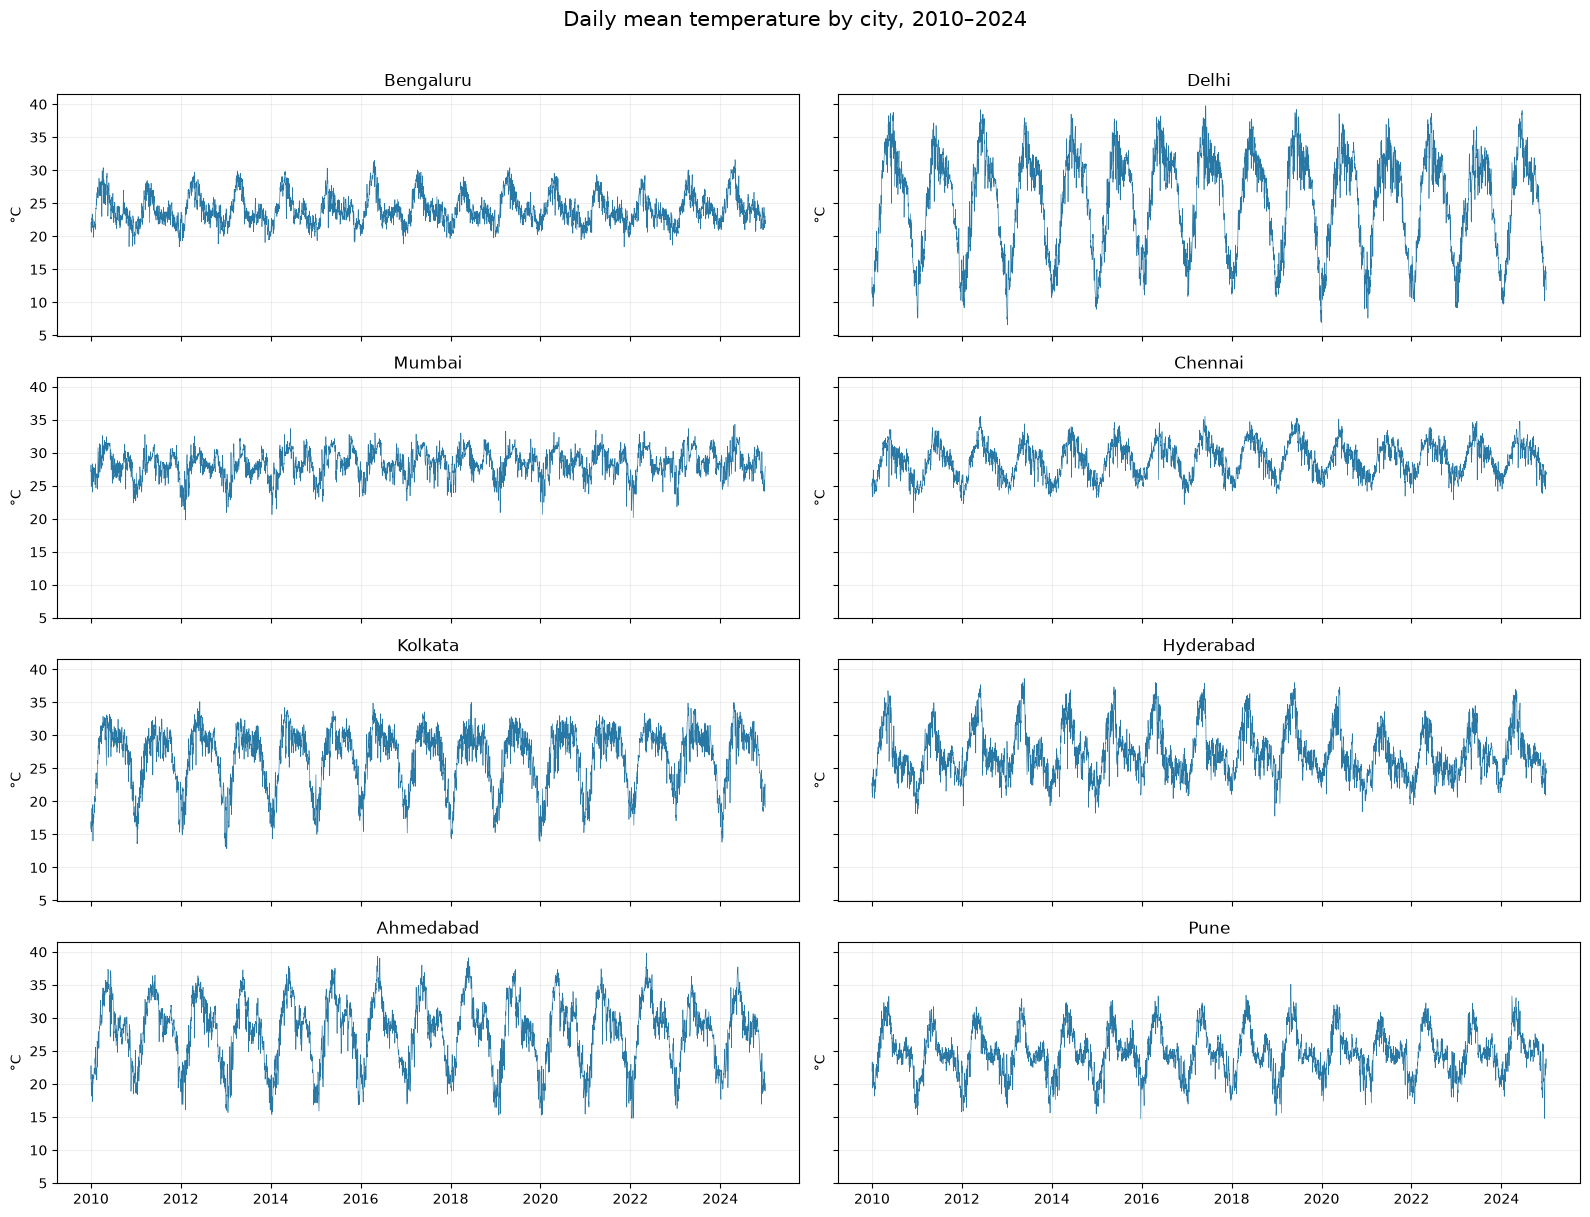
\includegraphics[width=\linewidth]{eight_city_daily_temperature.png}
\caption{Daily mean temperature (interpolated series) at the eight stations, 2010--2024, on a shared vertical axis. Extracted from the executed eight-city notebook, Section~3.}
\label{fig:city_series}
\end{figure}

\begin{figure}[p]
\centering
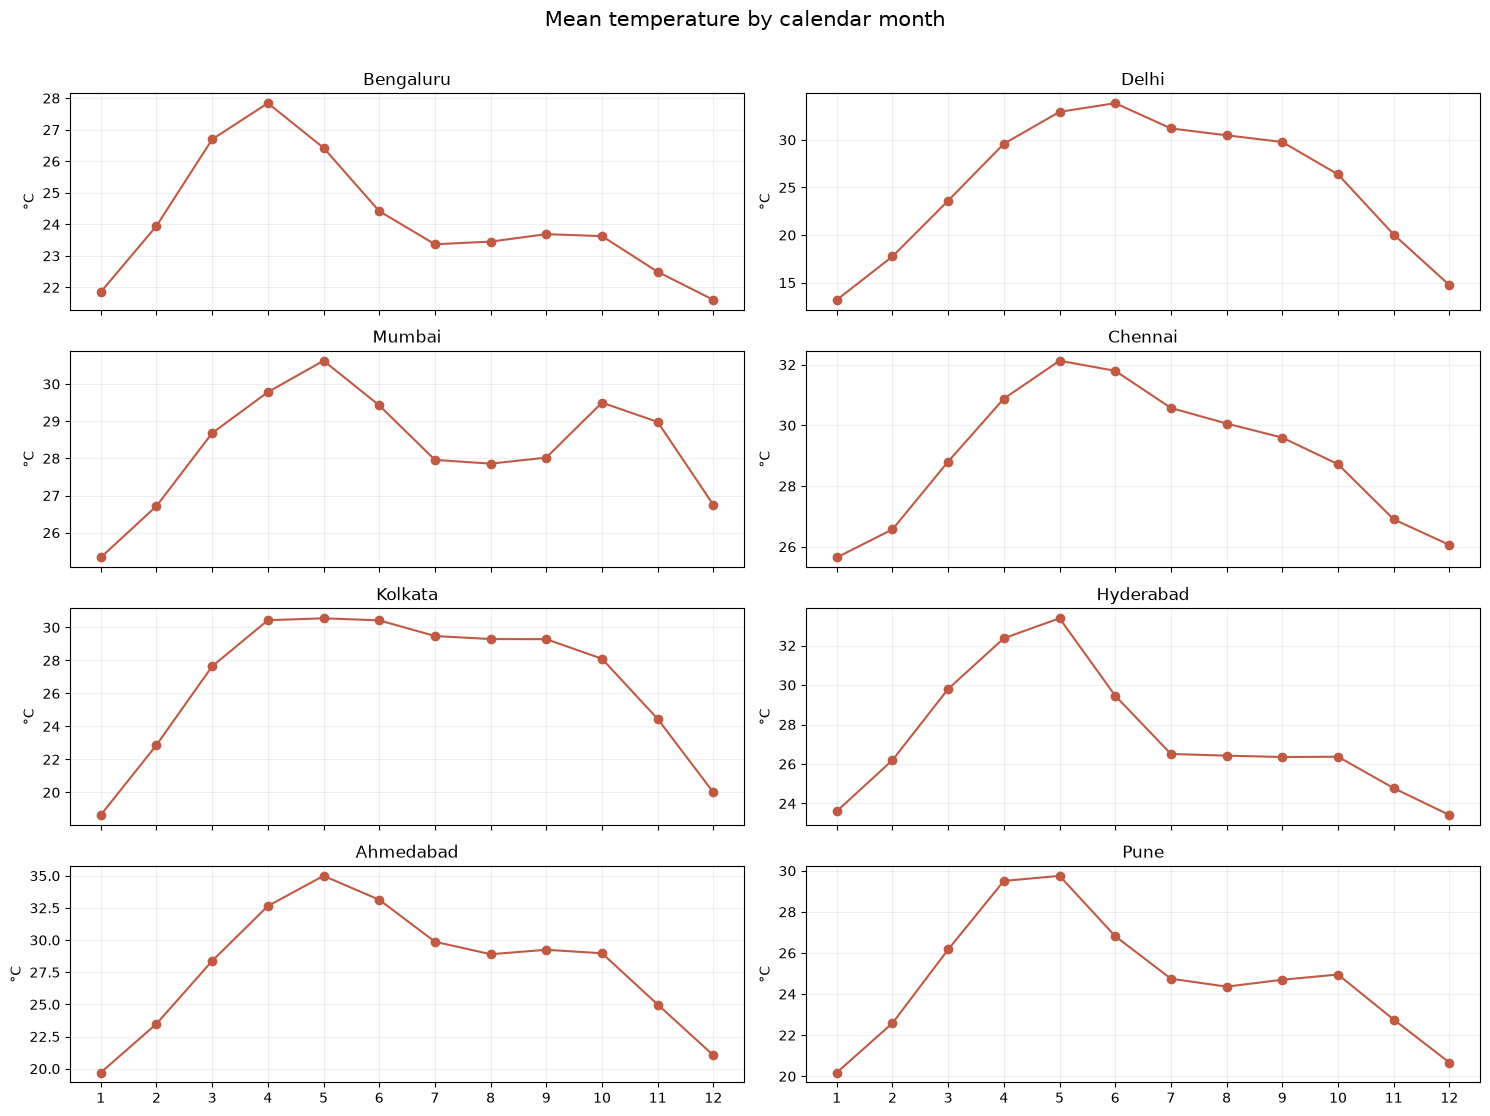
\includegraphics[width=\linewidth]{eight_city_monthly_climatology.png}
\caption{Mean daily temperature by calendar month, 2010--2024. Each panel has its own vertical scale, so the shapes are comparable but the amplitudes should be read from \cref{tab:descriptive}.}
\label{fig:climatology}
\end{figure}

\begin{table}[ht]
\centering
\small
\caption{Descriptive statistics of daily mean temperature, 2010--2024 (\si{\degreeCelsius}). Mean, SD, minimum and maximum use measured days only. Amplitude is the warmest minus the coolest monthly mean. Mean $|\Delta y|$ is the average absolute change between consecutive days.}
\label{tab:descriptive}
\begin{tabular}{@{}l r r r r l l r r@{}}
\toprule
City & Mean & SD & Min & Max & Warmest month & Coolest month & Amplitude & Mean $|\Delta y|$ \\
\midrule
\tabfile{tables/r1_descriptive.tex}
\bottomrule
\end{tabular}
\end{table}

All eight stations show an annual cycle, but its size and shape vary widely. Delhi swings from a January mean of 13.2\degC{} to a June mean of 33.9\degC{}, an amplitude of 20.7\degC; Ahmedabad (15.3\degC) and Kolkata (11.9\degC) follow. The two coastal stations and Bengaluru have the narrowest cycles: Mumbai 5.3\degC, Bengaluru 6.2\degC{} and Chennai 6.5\degC. The timing is broadly shared: six stations peak in May, Delhi in June and Bengaluru in April, in each case before the monsoon rains arrive. Several climatologies are flat or double-peaked after the peak. Mumbai has a second maximum in October (\cref{fig:climatology}), after the monsoon withdraws, and Bengaluru, Hyderabad and Pune hold an almost constant level from July to October.

Day-to-day variability does not follow the same ordering as the annual amplitude. The mean absolute daily change is smallest at Chennai (0.62\degC), Mumbai (0.64\degC) and Bengaluru (0.67\degC) and largest at Delhi (1.13\degC), Hyderabad (0.95\degC) and Kolkata (0.93\degC). Hyderabad has only the fourth-largest seasonal amplitude but the second-largest daily change, which suggests that a city's annual range and its short-term variability need to be considered separately.

The single-station diagnostics for Bengaluru are shown in \cref{fig:bengaluru_eda}. The 30-day rolling standard deviation is itself seasonal, larger in the transition months, so the variance of the series is not constant even though its level is bounded. The subseries plot shows that each month's mean varies little from year to year around its long-run value, which is what a stable, regular seasonal cycle looks like.

\begin{figure}[ht]
\centering
\begin{subfigure}{\linewidth}
  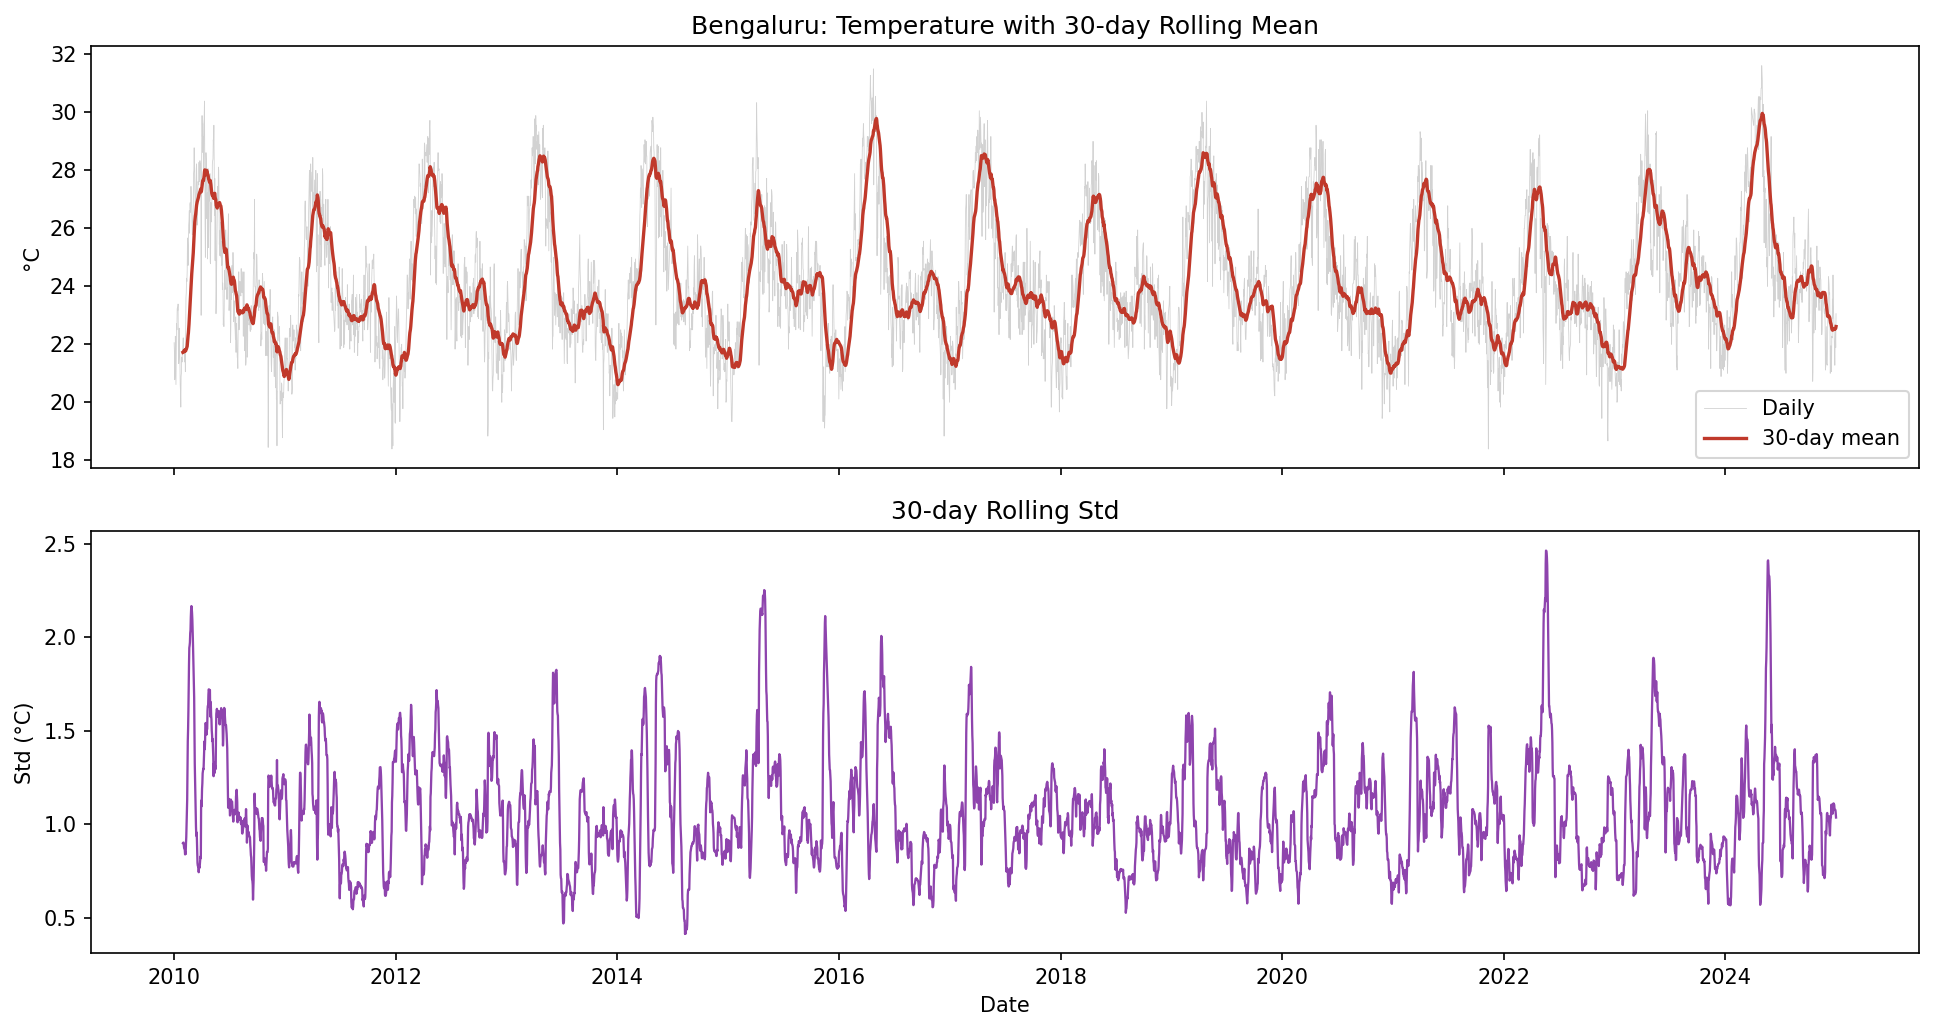
\includegraphics[width=\linewidth]{bengaluru_rolling_statistics.png}
  \caption{Daily series with 30-day rolling mean (top) and 30-day rolling standard deviation (bottom).}
\end{subfigure}\\[4pt]
\begin{subfigure}{\linewidth}
  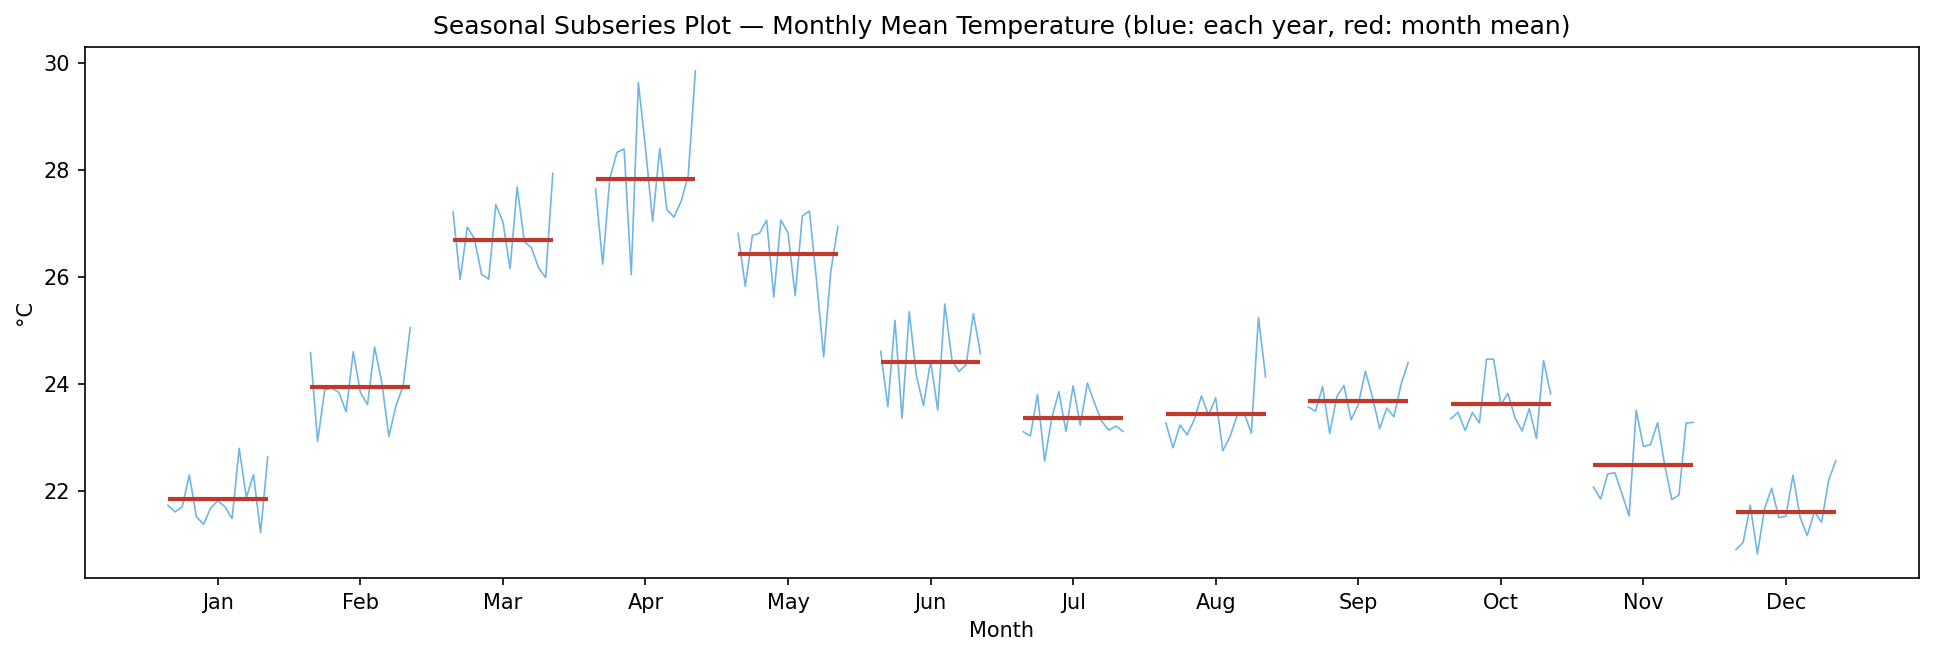
\includegraphics[width=\linewidth]{bengaluru_subseries.png}
  \caption{Seasonal subseries: per-year monthly means (blue) and the 2010--2024 monthly mean (red).}
\end{subfigure}
\caption{Bengaluru, the station of the original single-city study: rolling statistics and seasonal subseries.}
\label{fig:bengaluru_eda}
\end{figure}

\subsection{Trend}

\begin{table}[ht]
\centering
\small
\caption{Seasonal and trend summaries. $F_S$ and $F_T$ follow \cref{eq:strength}. The OLS slope is fitted to the daily series; the STL change is the last minus the first value of the STL trend component. ``Same sign'' indicates whether the two trend estimates agree in direction.}
\label{tab:trend}
\begin{tabular}{@{}l r r r r c r@{}}
\toprule
City & $F_S$ & $F_T$ & OLS slope (\si{\degreeCelsius}/decade) & STL change (\si{\degreeCelsius}) & Same sign & ACF lag 365 \\
\midrule
\tabfile{tables/r1_trend_season.tex}
\bottomrule
\end{tabular}
\end{table}

\Cref{tab:trend} gives no consistent picture of a trend. Trend strength is low everywhere ($F_T$ = 0.06--0.18), and the two trend estimates point in opposite directions for five stations: Delhi, Mumbai, Kolkata, Hyderabad and Pune. Delhi illustrates why (\cref{fig:delhi_stl}): its STL trend component falls from about 26.3\degC{} in 2010 to a low in 2011--2013, rises to a peak in late 2016 and then falls back, so the endpoint difference is $-0.92$\degC{} while the least-squares line through all fifteen years is almost flat ($+0.06$\degC{} per decade). Both estimators are sensitive to the start and end of a fifteen-year record, and neither was accompanied by a significance test. Only Bengaluru, Chennai and Ahmedabad show agreeing signs; Chennai's estimates are the largest ($+0.77$\degC{} per decade and $+0.94$\degC{} over the record).

We therefore do not claim a warming (or cooling) trend for these cities. The original single-station report described Bengaluru's $+0.19$\degC{} per decade as a mild warming trend; the eight-city comparison shows that estimates of this size change sign across estimators at most stations, so that description is too strong without a formal trend test over a longer record. For forecasting, the relevant point is the magnitude: even the largest slope (Chennai's) amounts to about 1.2\degC{} over the fifteen years, against seasonal amplitudes of 5--21\degC.

\begin{figure}[ht]
\centering
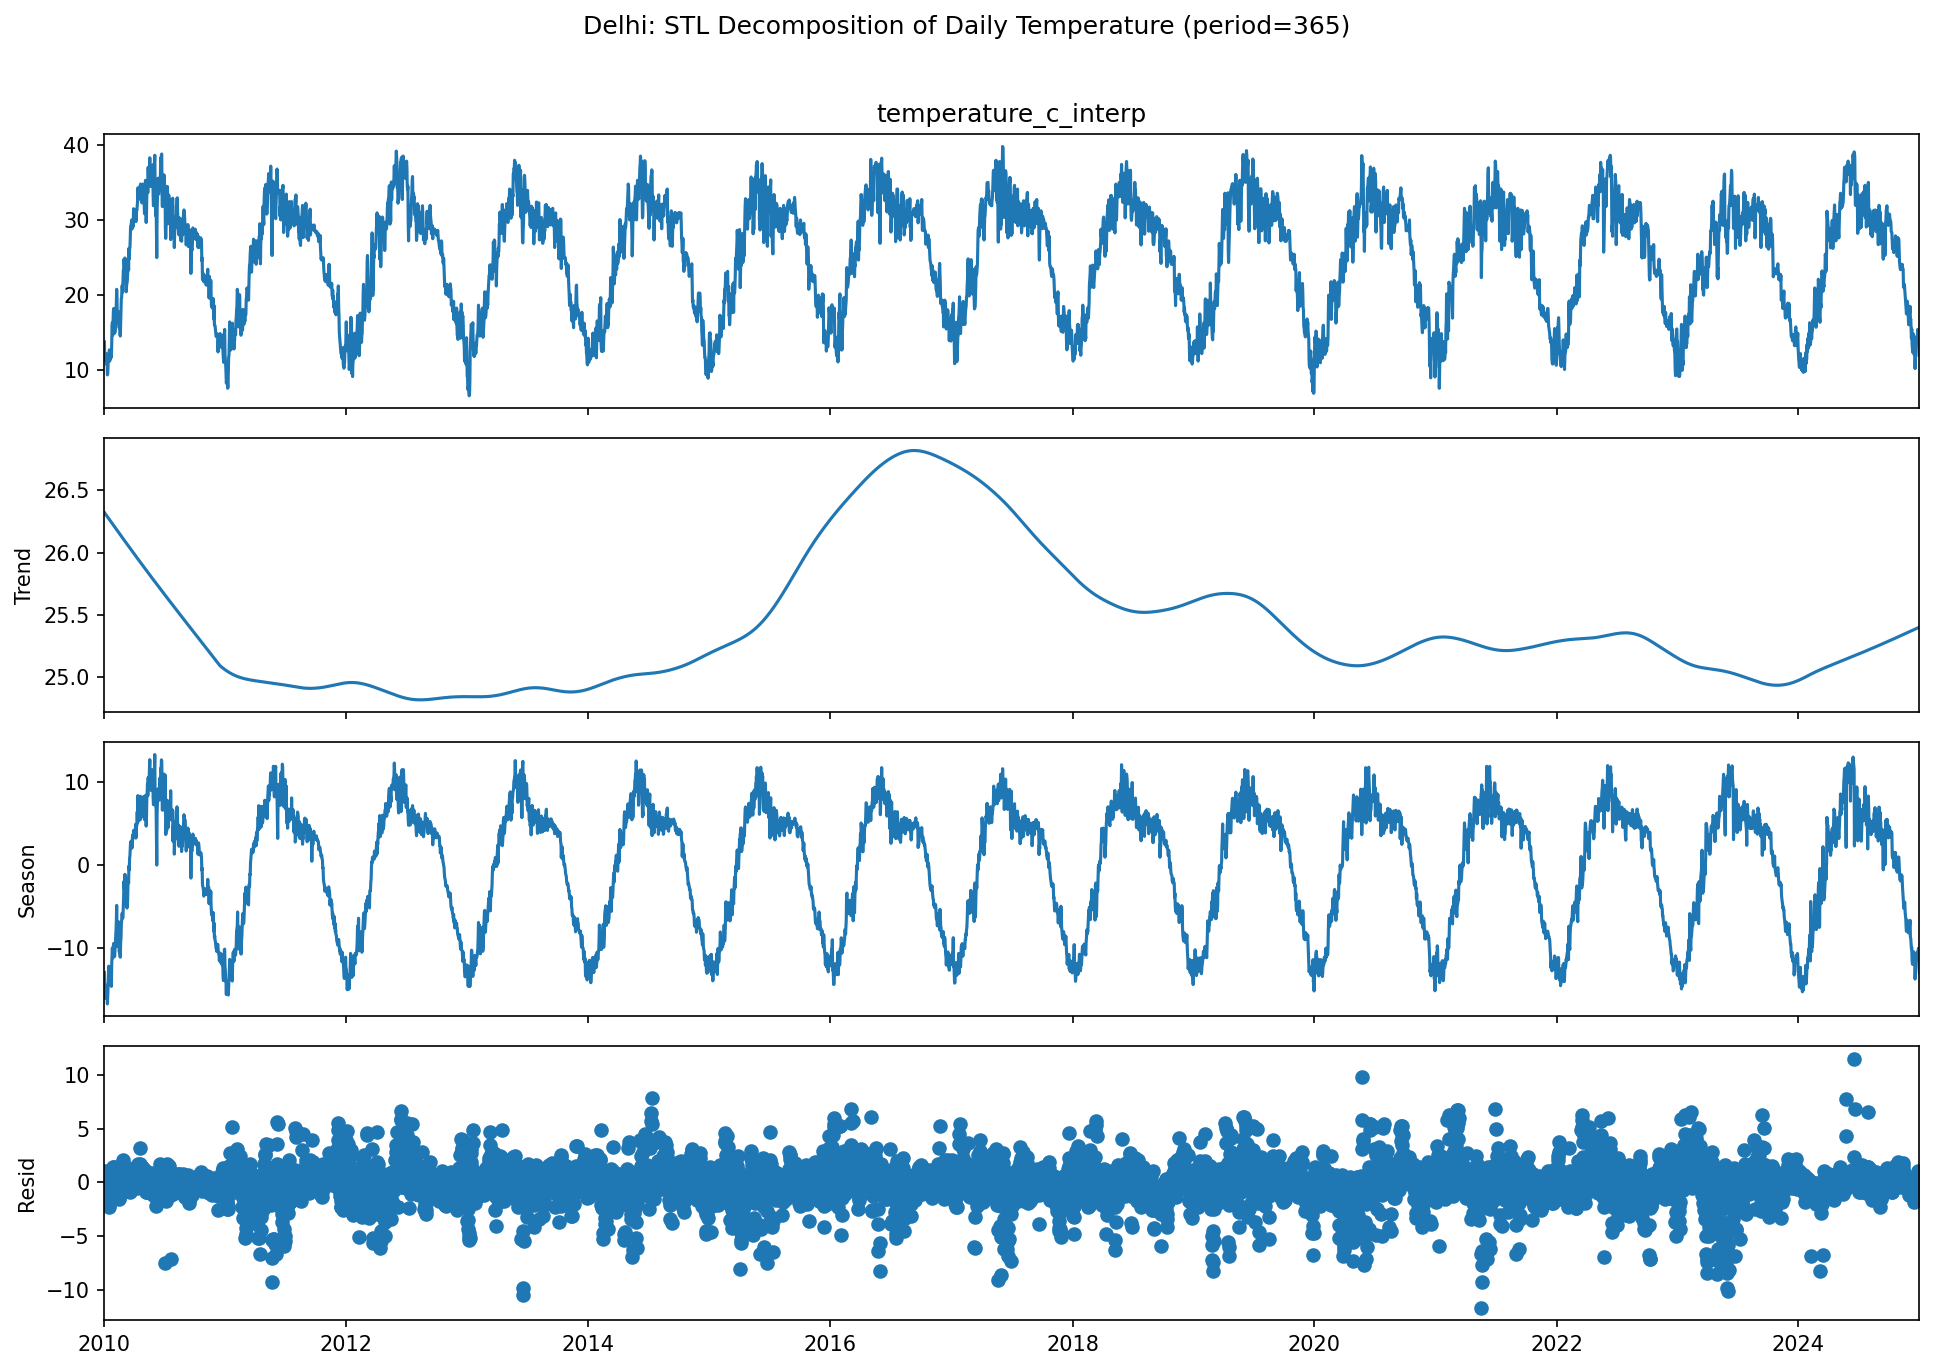
\includegraphics[width=0.92\linewidth]{delhi_stl.png}
\caption{STL decomposition (period 365, robust) of Delhi's daily mean temperature. The trend panel spans only about 2\degC{} and is not monotonic; the seasonal panel dominates.}
\label{fig:delhi_stl}
\end{figure}

\subsection{Seasonality}

The seasonal strength $F_S$ ranges from 0.64 at Mumbai to 0.93 at Delhi (\cref{tab:trend}). Seven stations are at or above 0.80. The ordering is close to the ordering of the annual amplitudes in \cref{tab:descriptive}, as expected, since a larger seasonal swing makes $\operatorname{Var}(S_t)$ larger relative to $\operatorname{Var}(R_t)$. Mumbai is the outlier at the low end: its small, double-peaked cycle explains a smaller share of the daily variation than at any other station.

The autocorrelation at lag 365 gives independent evidence of the same cycle (\cref{fig:longlag}). It ranges from 0.58 (Mumbai) to 0.91 (Delhi), and in every panel the long-lag ACF turns negative within the year and peaks again at lag 364--366. The position of the negative minimum varies: it lies between lags 180 and 255 at seven stations but at lag 95 for Mumbai, whose double-peaked climatology puts two warm seasons into each year. The cycle is regular rather than erratic: in the subseries plots, the year-to-year scatter of each monthly mean is small compared with the differences between months (\cref{fig:bengaluru_eda}).

\begin{figure}[p]
\centering
\begin{subfigure}{0.49\linewidth}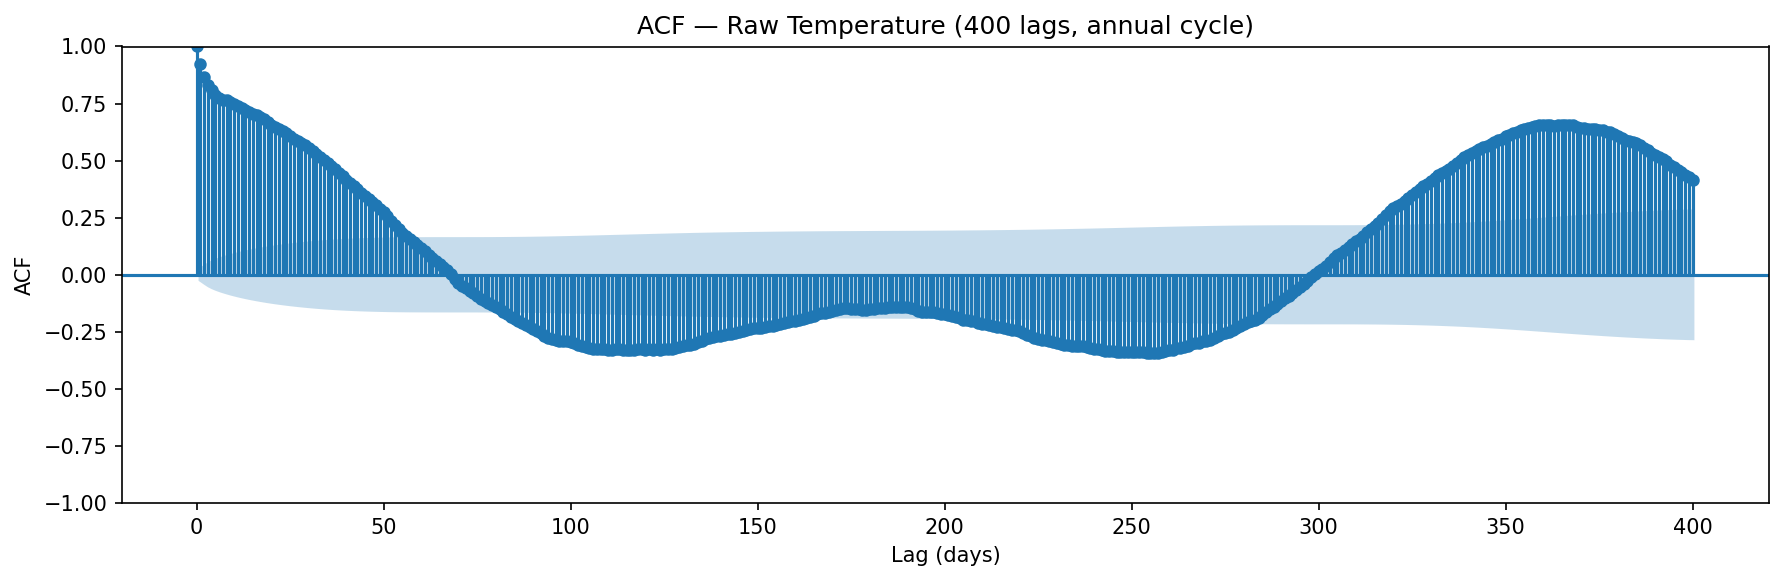
\includegraphics[width=\linewidth]{acf_longlag_bengaluru.png}\caption{Bengaluru}\end{subfigure}\hfill
\begin{subfigure}{0.49\linewidth}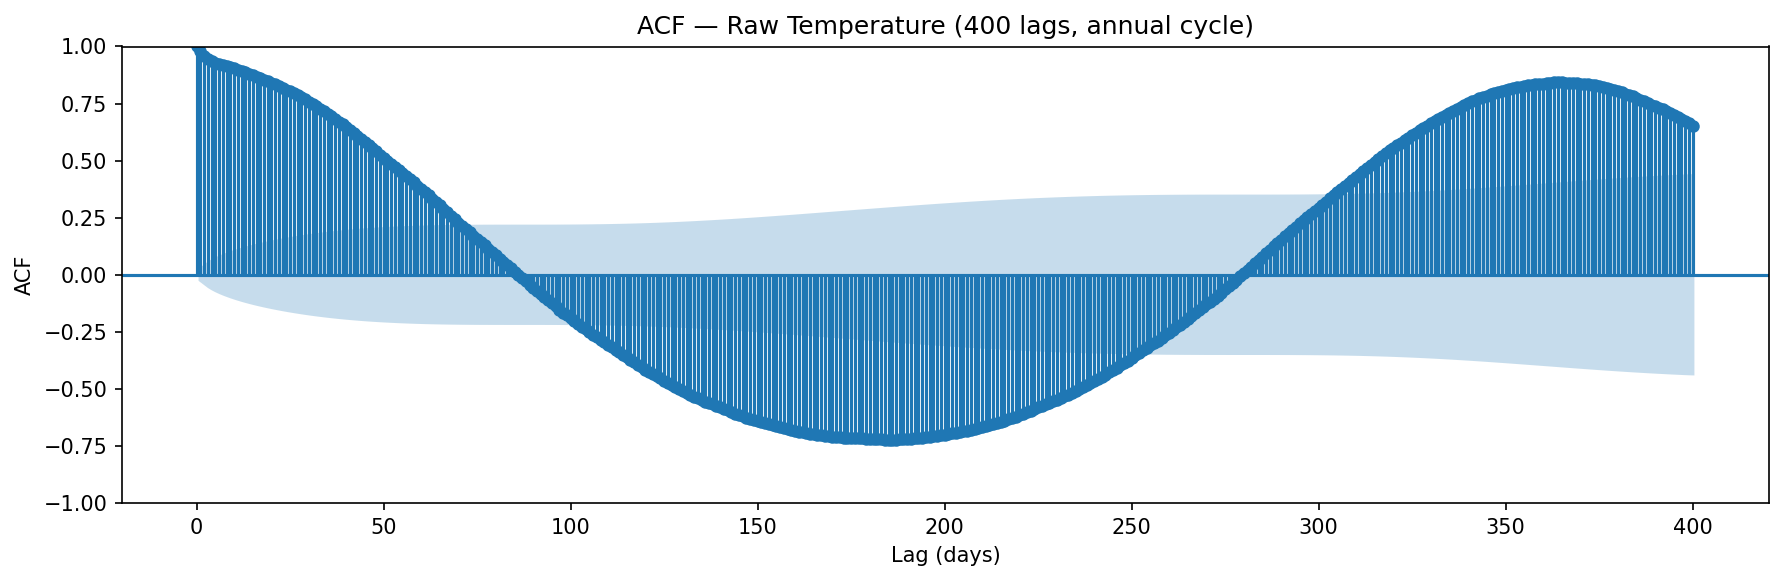
\includegraphics[width=\linewidth]{acf_longlag_delhi.png}\caption{Delhi}\end{subfigure}\\[3pt]
\begin{subfigure}{0.49\linewidth}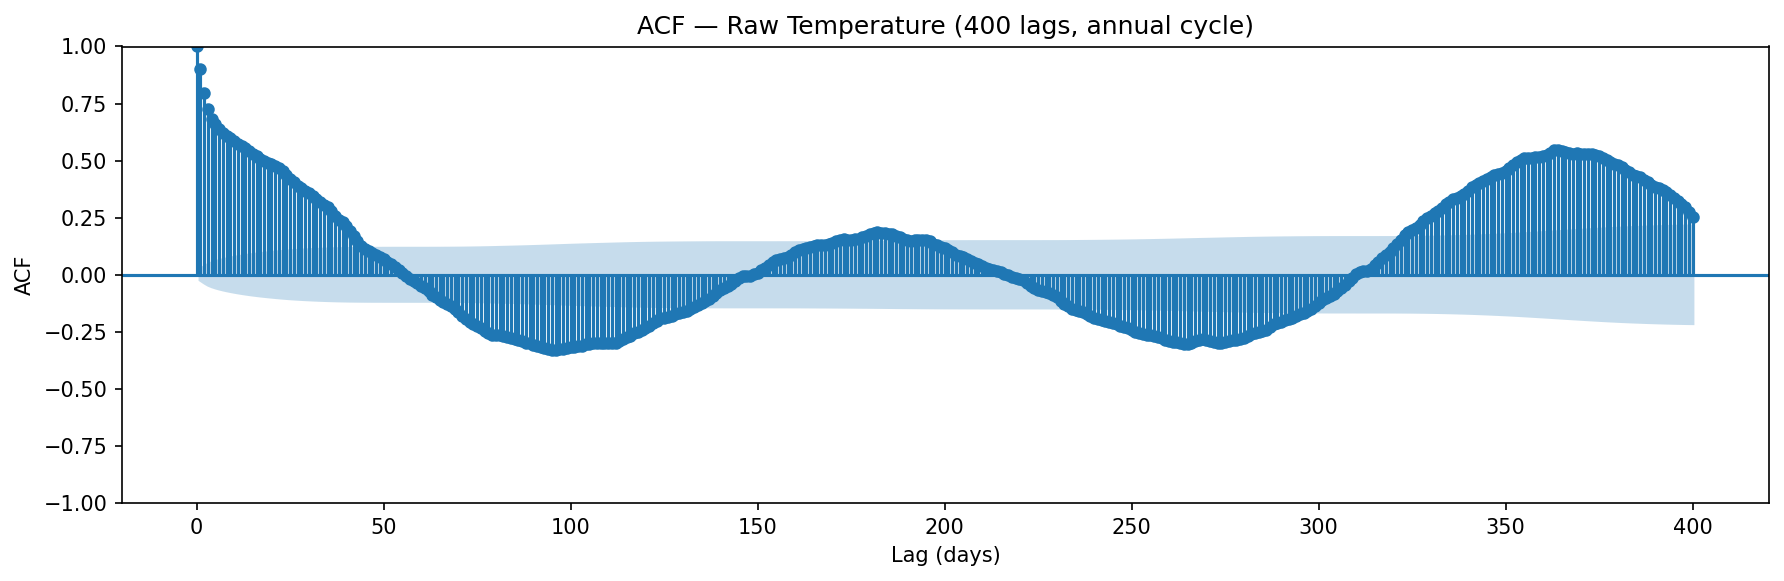
\includegraphics[width=\linewidth]{acf_longlag_mumbai.png}\caption{Mumbai}\end{subfigure}\hfill
\begin{subfigure}{0.49\linewidth}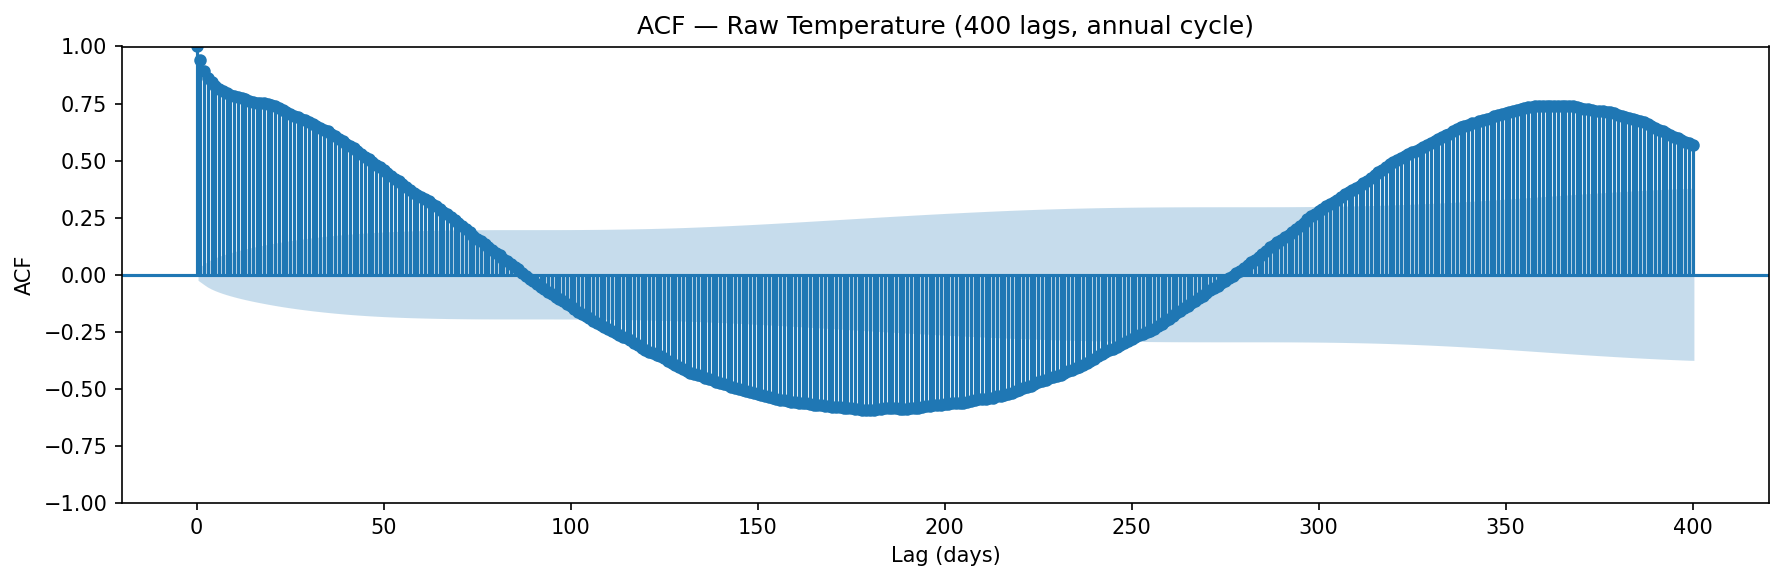
\includegraphics[width=\linewidth]{acf_longlag_chennai.png}\caption{Chennai}\end{subfigure}\\[3pt]
\begin{subfigure}{0.49\linewidth}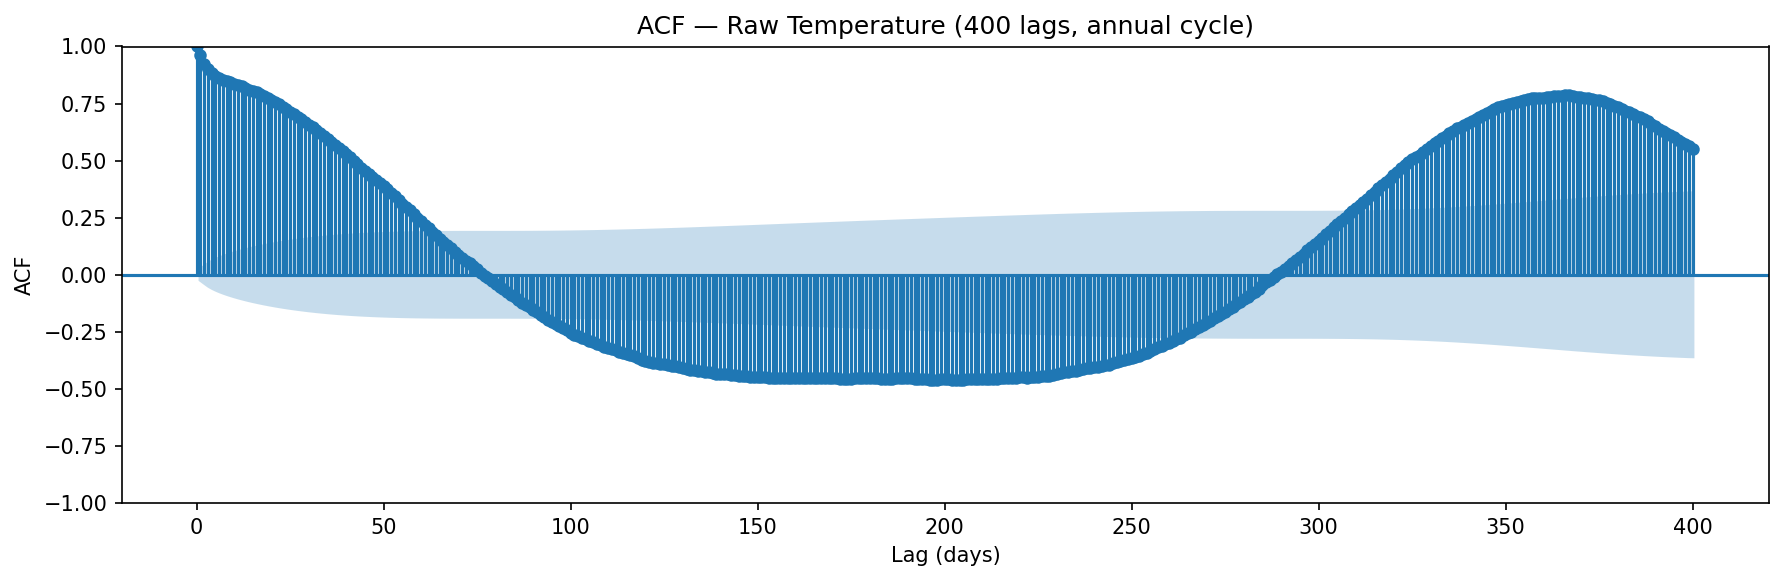
\includegraphics[width=\linewidth]{acf_longlag_kolkata.png}\caption{Kolkata}\end{subfigure}\hfill
\begin{subfigure}{0.49\linewidth}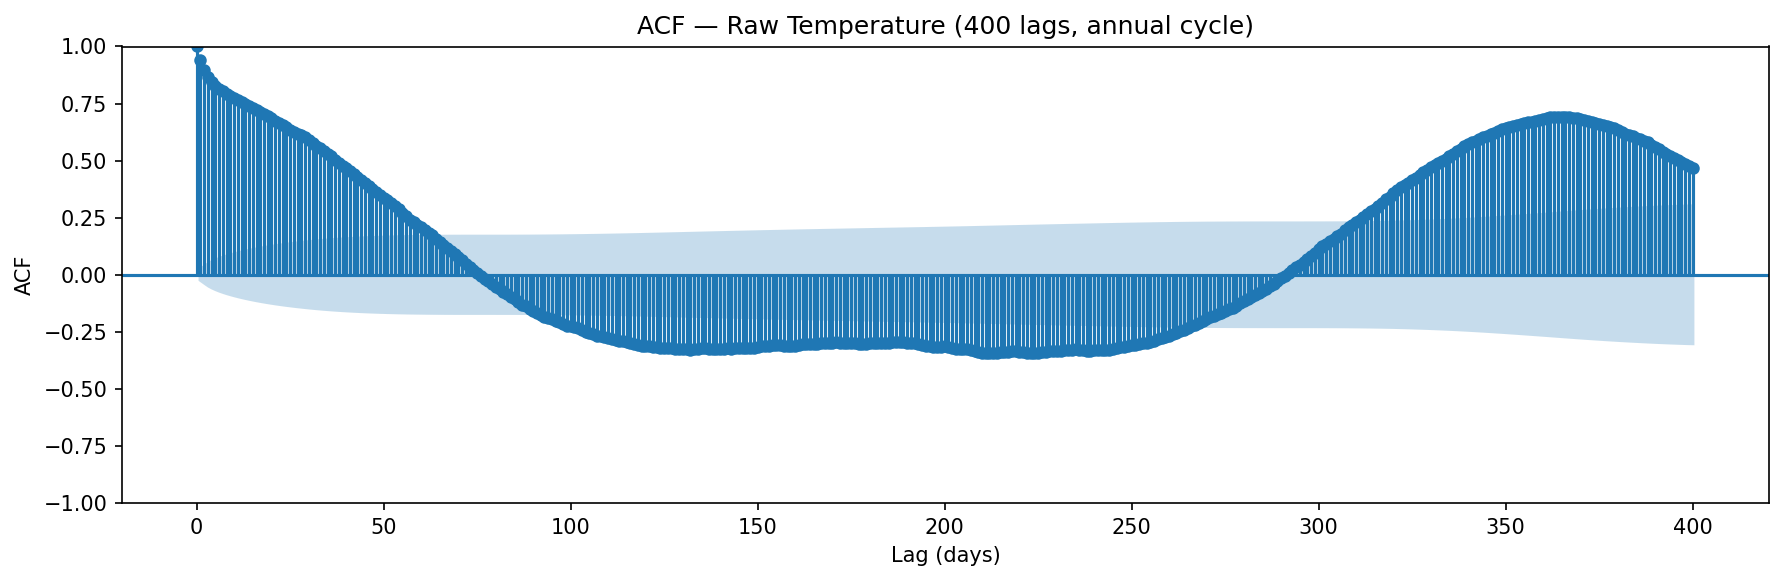
\includegraphics[width=\linewidth]{acf_longlag_hyderabad.png}\caption{Hyderabad}\end{subfigure}\\[3pt]
\begin{subfigure}{0.49\linewidth}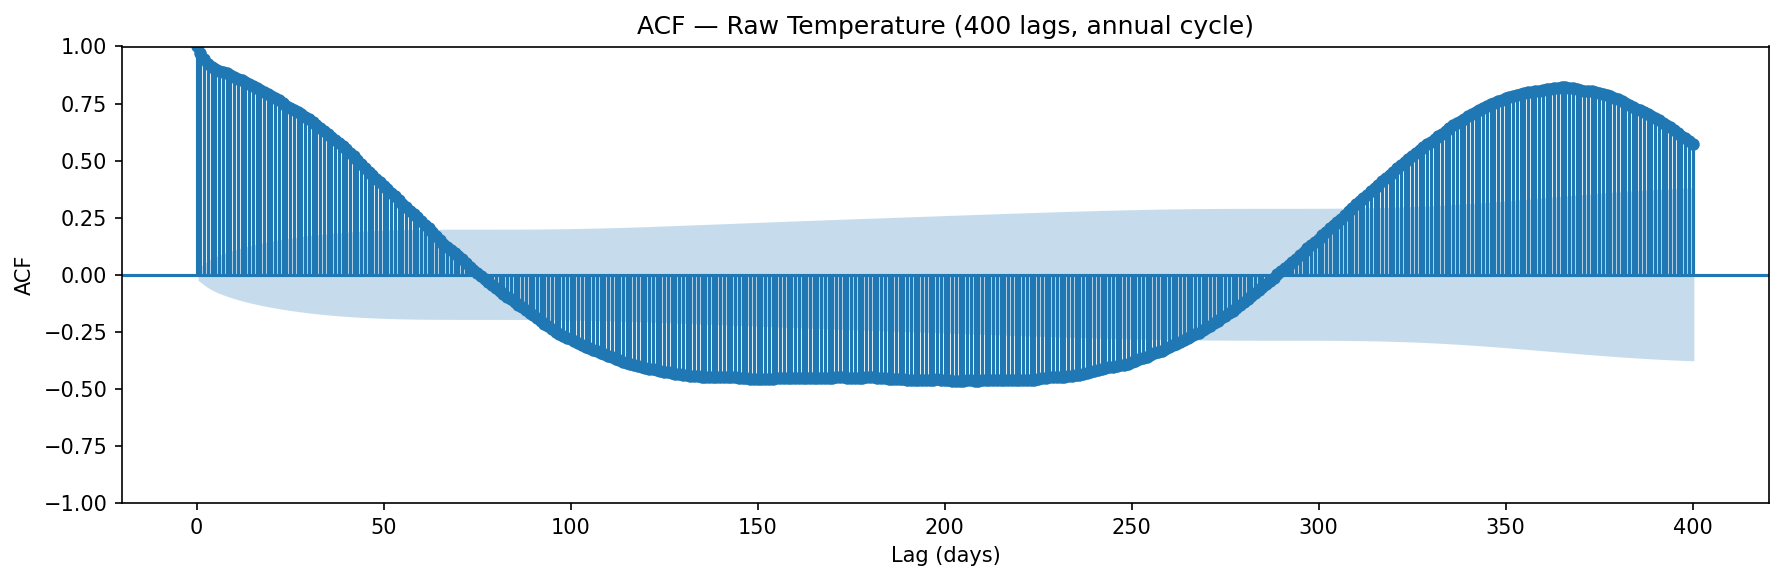
\includegraphics[width=\linewidth]{acf_longlag_ahmedabad.png}\caption{Ahmedabad}\end{subfigure}\hfill
\begin{subfigure}{0.49\linewidth}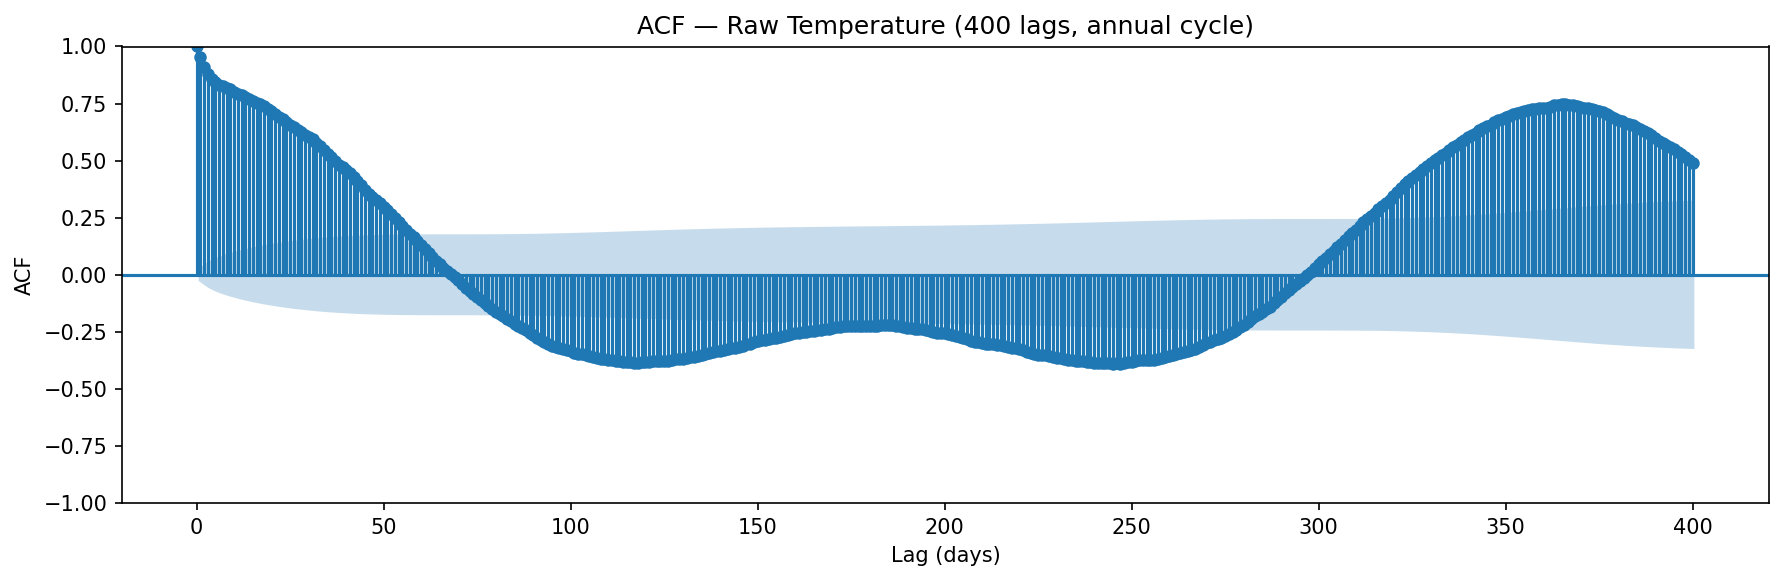
\includegraphics[width=\linewidth]{acf_longlag_pune.png}\caption{Pune}\end{subfigure}
\caption{Autocorrelation of the level series to lag 400 (shaded: approximate 95\% band). Every station has a negative trough within the year and a second peak at lag 364--366, the signature of the annual cycle.}
\label{fig:longlag}
\end{figure}

\subsection{Stationarity}

\begin{table}[ht]
\centering
\small
\caption{ADF and KPSS tests on the level series and its first difference (full 2010--2024 interpolated series). 5\% critical values: ADF $-2.86$; KPSS 0.463.}
\label{tab:stationarity}
\begin{tabular}{@{}l rr rr rr rr@{}}
\toprule
 & \multicolumn{4}{c}{Level $y_t$} & \multicolumn{4}{c}{First difference $\Delta y_t$} \\
\cmidrule(lr){2-5}\cmidrule(l){6-9}
City & ADF & $p$ & KPSS & $p$ & ADF & $p$ & KPSS & $p$ \\
\midrule
\tabfile{tables/r1_stationarity.tex}
\bottomrule
\end{tabular}
\end{table}

The two tests agree at every station (\cref{tab:stationarity}). ADF rejects the unit-root null for the level series (statistics from $-4.42$ to $-8.34$, all $p \leq 0.0003$), and KPSS does not reject level stationarity. Mumbai comes closest to a KPSS rejection: its statistic of 0.404 is below the 5\% critical value of 0.463, with $p = 0.076$. Differencing leaves the conclusion unchanged and moves the ADF statistic much further from zero.

Physically, a bounded variable that returns to the same seasonal level each year would be expected to behave this way; daily temperature does not wander like a random walk. Two qualifications matter for how this result is used. First, the tests were run with a constant only, so the deterministic annual cycle is absorbed into what the tests treat as stationary fluctuation. ``Stationary'' here means that there is no stochastic trend; it does not mean that the mean is constant through the year. Second, KPSS with an automatic bandwidth of about 40 lags has limited power against slow, persistent departures, so its failure to reject is weaker evidence than ADF's rejection.

These results answer the differencing question for later modelling: with no unit root, $d = 0$ is appropriate, and first differencing would only add a non-invertible moving-average component. Differencing does change the correlation structure (\cref{sec:acf}), which is why we report it. No variance-stabilising transformation was applied to temperature: it is an interval-scale quantity with a bounded, roughly symmetric range, and a logarithm has no physical meaning for it. Precipitation, which is strongly right-skewed (\cref{sec:precip}), would warrant a $\log(1+P)$ transform if it were ever modelled directly.

\subsection{Autocorrelation and partial autocorrelation}
\label{sec:acf}

\begin{table}[ht]
\centering
\small
\caption{Autocorrelation summaries on the full 2010--2024 series. ACF values on the level series and the differenced series; PACF on the level series. The 95\% white-noise band is $\pm 0.026$.}
\label{tab:acf}
\begin{tabular}{@{}l rrr rrr r@{}}
\toprule
 & \multicolumn{3}{c}{ACF, level} & \multicolumn{3}{c}{PACF, level} & ACF, $\Delta y_t$ \\
\cmidrule(lr){2-4}\cmidrule(lr){5-7}\cmidrule(l){8-8}
City & lag 1 & lag 7 & lag 365 & lag 1 & lag 2 & lag 3 & lag 1 \\
\midrule
\tabfile{tables/r1_acf.tex}
\bottomrule
\end{tabular}
\end{table}

Persistence is the dominant short-range feature (\cref{tab:acf}). The lag-1 autocorrelation lies between 0.90 (Mumbai) and 0.98 (Delhi), and the ACF decays slowly over the following weeks without cutting off (\cref{fig:bengaluru_corr}a). A slow, smooth decay of this kind is what an autoregressive process superimposed on a deterministic annual cycle produces; it is not the pattern of a short moving-average process.

The PACF has one dominant spike at lag 1 equal to the lag-1 ACF, followed by much smaller values: at lags 2 and 3 none exceeds 0.15 in absolute value (\cref{tab:acf}, \cref{fig:bengaluru_corr}b). With 5{,}479 observations the 95\% band is narrow ($\pm 0.026$), so several of these small partial autocorrelations are statistically detectable without being large. Most of today's predictable information about tomorrow therefore comes from today. The remaining partial autocorrelation at lags 2--7 is consistent with the annual cycle, which a single autoregressive lag cannot represent; whether it vanishes once the cycle is removed is a question for the model identification in Review 2.

Differencing removes the persistence almost entirely. The lag-1 ACF of $\Delta y_t$ ranges from $-0.15$ (Bengaluru) to $+0.03$ (Mumbai), and the slow decay disappears (\cref{fig:bengaluru_corr}c,d). It is negative at six of the eight stations, most clearly at Bengaluru, Hyderabad and Chennai, which is consistent with differencing a series that was already stationary and supports $d = 0$.

\begin{figure}[ht]
\centering
\begin{subfigure}{0.49\linewidth}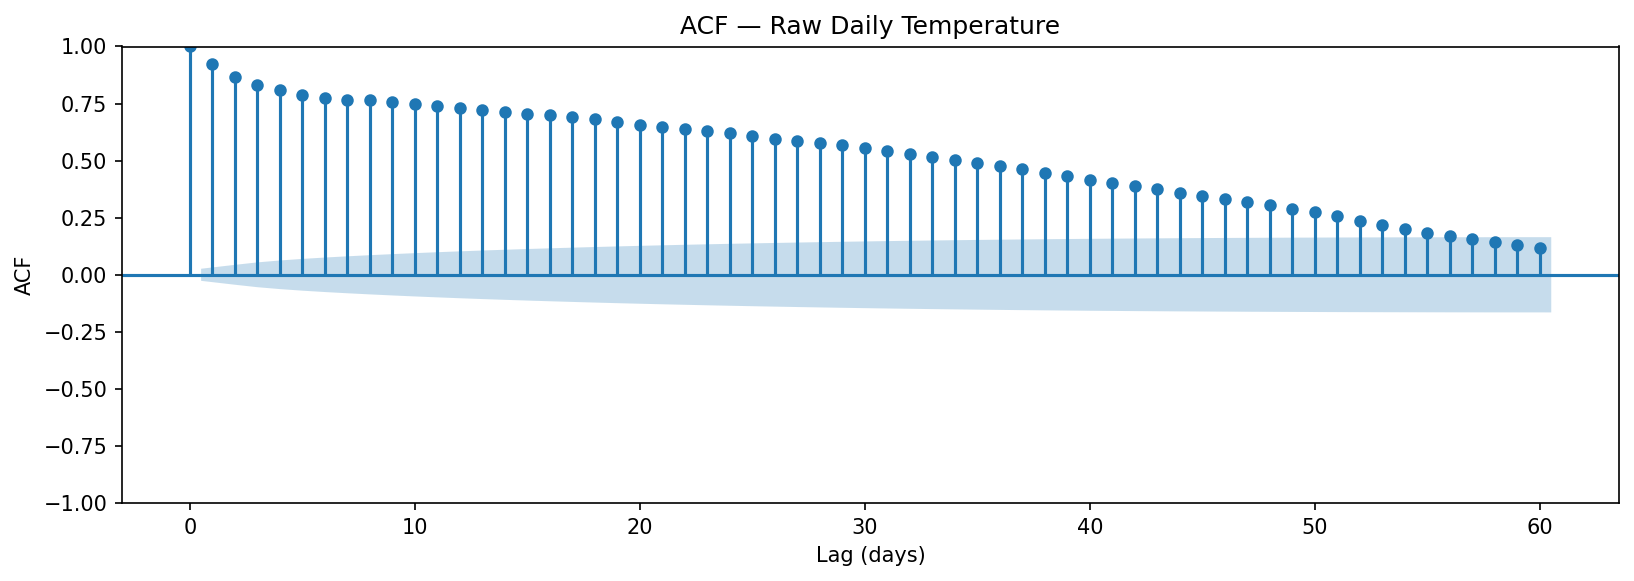
\includegraphics[width=\linewidth]{bengaluru_acf_raw.png}\caption{ACF, level}\end{subfigure}\hfill
\begin{subfigure}{0.49\linewidth}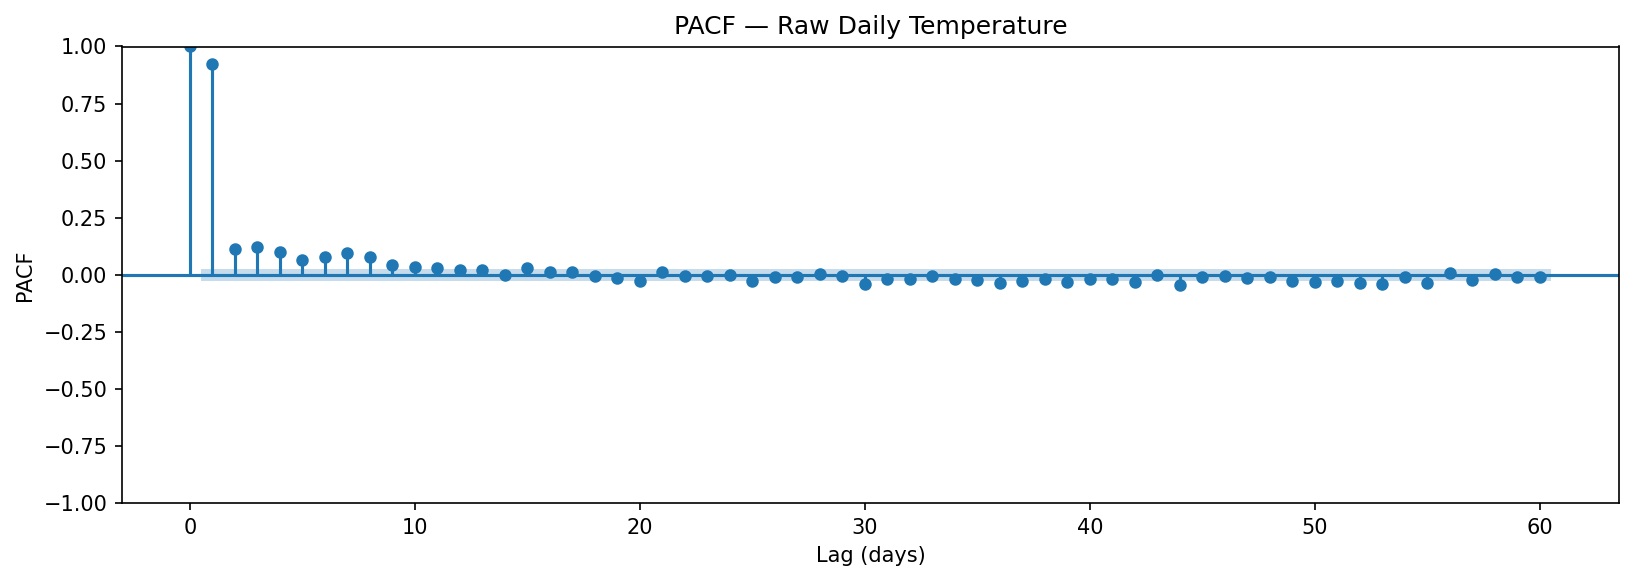
\includegraphics[width=\linewidth]{bengaluru_pacf_raw.png}\caption{PACF, level}\end{subfigure}\\[3pt]
\begin{subfigure}{0.49\linewidth}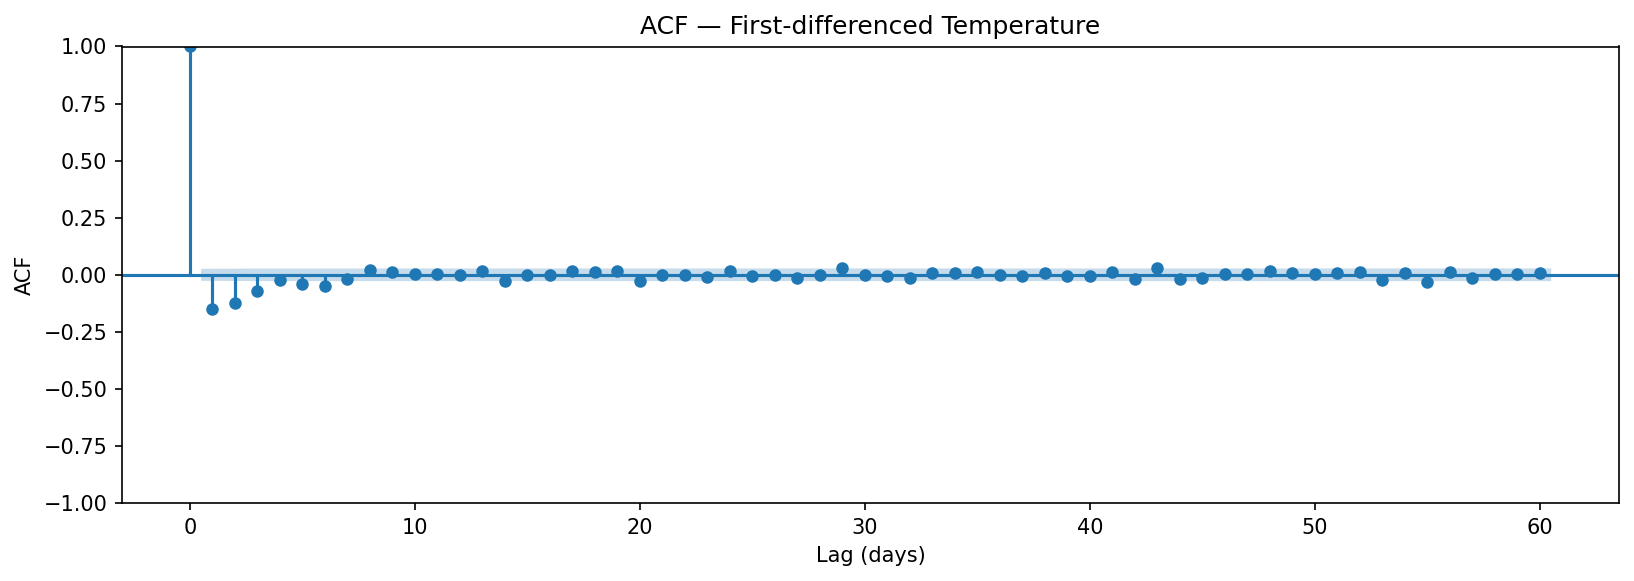
\includegraphics[width=\linewidth]{bengaluru_acf_diff.png}\caption{ACF, first difference}\end{subfigure}\hfill
\begin{subfigure}{0.49\linewidth}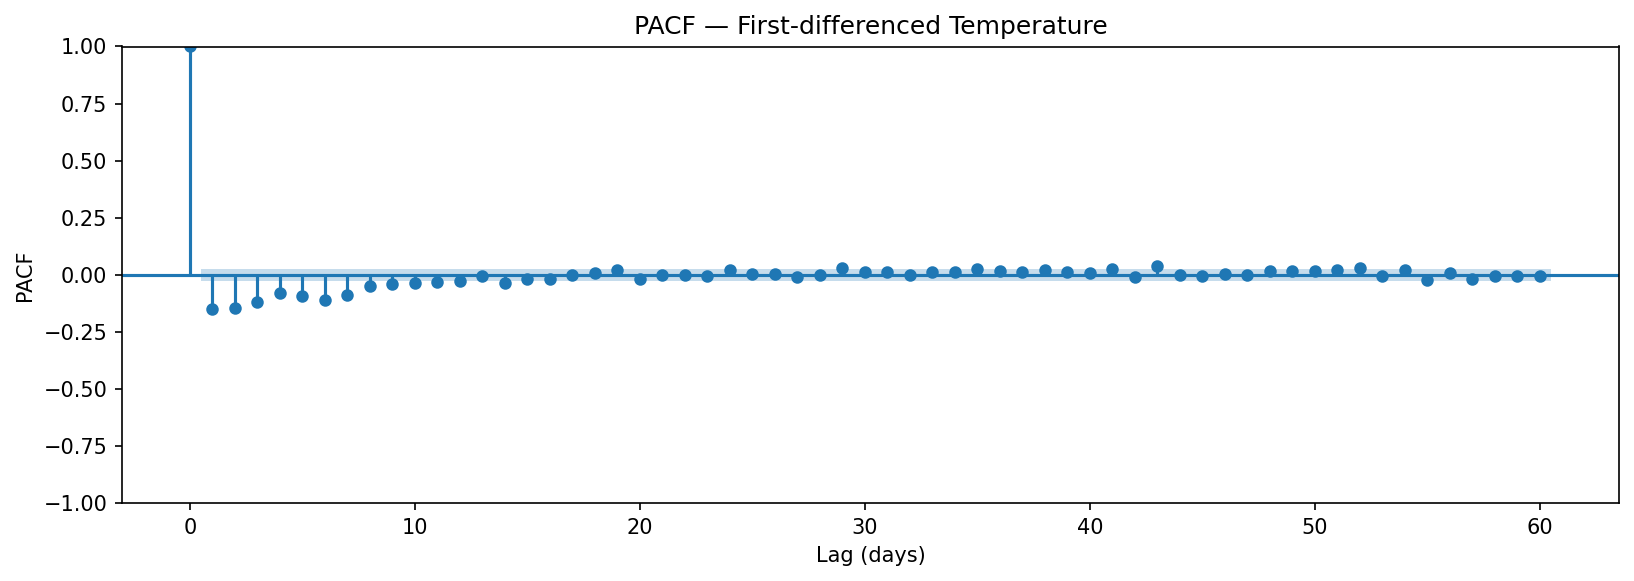
\includegraphics[width=\linewidth]{bengaluru_pacf_diff.png}\caption{PACF, first difference}\end{subfigure}
\caption{Correlograms for Bengaluru to lag 60. The equivalent figures for the other seven stations are in \code{figures/cities/<city>/} in the repository and follow the same pattern.}
\label{fig:bengaluru_corr}
\end{figure}

\subsection{Precipitation as a contrasting variable}
\label{sec:precip}

\begin{table}[ht]
\centering
\small
\caption{Daily precipitation after treating flag \code{I} as missing (mm). ``Wet'' is the share of measured days with a non-zero total.}
\label{tab:precip}
\begin{tabular}{@{}l r r r r r r@{}}
\toprule
City & Measured days & Missing (\%) & Wet (\%) & Median & Mean & Max \\
\midrule
\tabfile{tables/r1_precip.tex}
\bottomrule
\end{tabular}
\end{table}

Precipitation behaves very differently from temperature (\cref{tab:precip}, \cref{fig:bengaluru_precip}). Between 47\% (Bengaluru) and 77\% (Ahmedabad) of days carry no usable measurement, most of them because of the \code{I} flag (at Kolkata about a fifth are instead the 99.99 missing code). The missing days are not a random sample: a station that reports no precipitation and notes none in its hourly observations is most likely to do so on dry days, so the measured days over-represent wet ones. The wet-day shares in \cref{tab:precip} (59--83\%) are therefore biased upward and should not be read as rainfall frequencies. Among measured days the distribution is extremely right-skewed. Mumbai, for example, has a median of 6.1\,mm, a mean of 21.4\,mm and a maximum of 374.9\,mm, and the means exceed the medians by a factor of 3.5 (Mumbai) to 12 (Bengaluru). In aggregate, rainfall follows the monsoon calendar (\cref{fig:bengaluru_precip}b), but from one day to the next it is intermittent and bursty. Combined with the missingness, this makes precipitation unsuitable as a forecasting target or input for this project, and we keep it as descriptive context.

\begin{figure}[ht]
\centering
\begin{subfigure}{0.58\linewidth}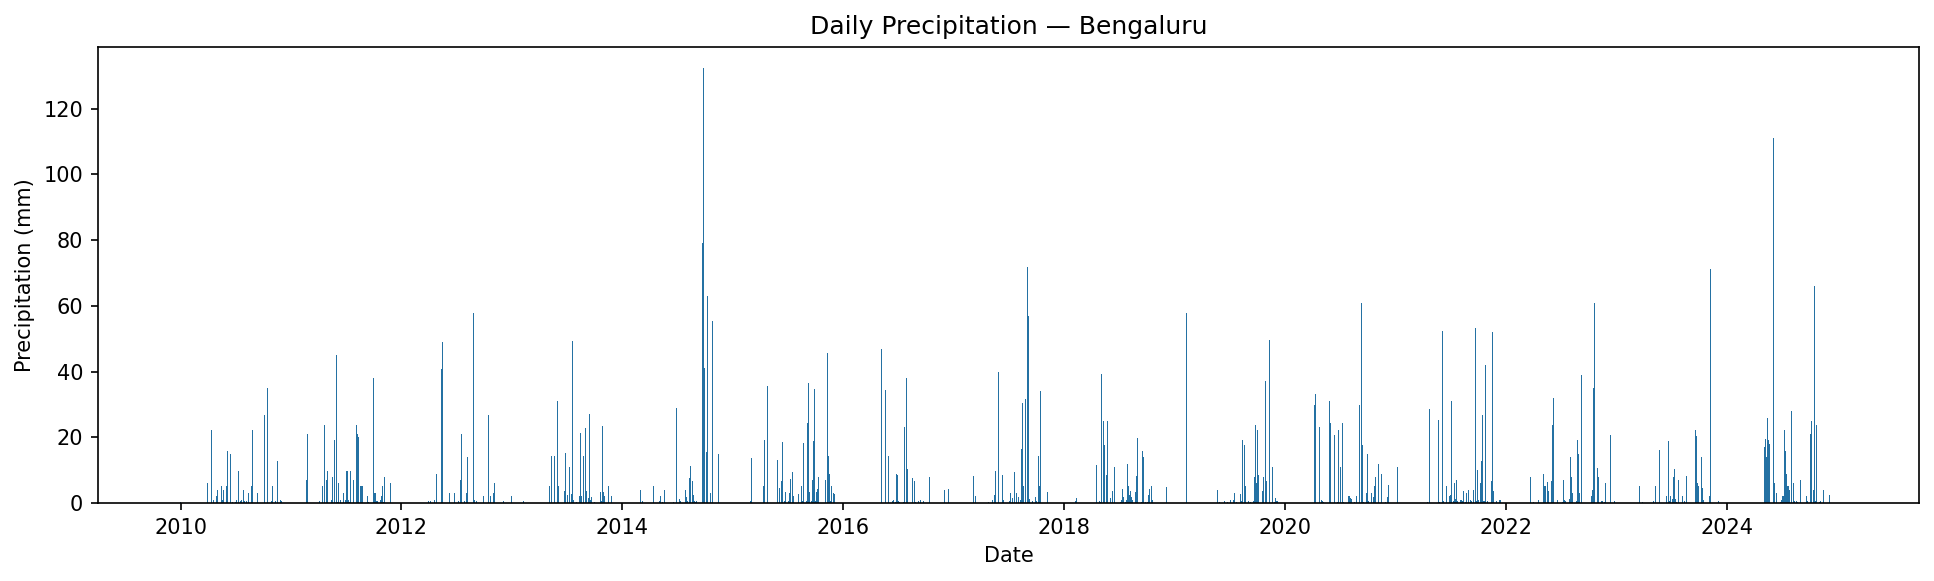
\includegraphics[width=\linewidth]{bengaluru_precipitation.png}\caption{Daily precipitation, measured days only}\end{subfigure}\hfill
\begin{subfigure}{0.40\linewidth}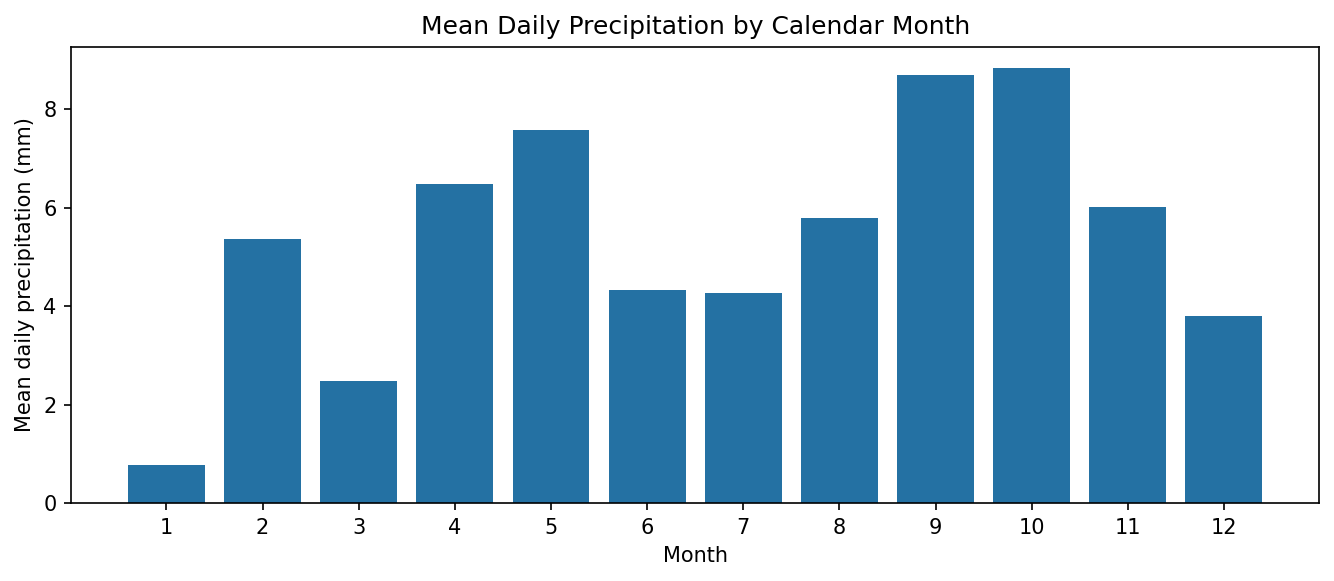
\includegraphics[width=\linewidth]{bengaluru_monthly_precipitation.png}\caption{Mean daily precipitation by month}\end{subfigure}
\caption{Precipitation at Bengaluru. Rainfall is concentrated in the monsoon and post-monsoon months, with long dry spells in between.}
\label{fig:bengaluru_precip}
\end{figure}

\section{Forecasting problem and design for Review 2}
\label{sec:forecast}

\paragraph{Target and horizons.} The forecast target is the daily mean temperature $y_{t+h}$ at each station. The primary task is one day ahead ($h = 1$), the horizon at which the persistence documented in \cref{sec:acf} is most useful. A secondary task covers leads of up to 30 days, to see how much each method gains or loses as the information in recent observations decays.

\paragraph{Evaluation design.} Each series is split chronologically into training (first 70\%), validation (next 15\%) and test (final 15\%) segments, without shuffling. For every station the test segment covers the same 822 days, 2 October 2022 to 31 December 2024, so that errors can be compared across cities over identical weather periods. Any scaling is fitted on the training segment only, and the test segment is used for nothing except final scoring. One caveat follows from \cref{sec:cleaning}: interpolated values lean on the next observed day, so the filled days (0.2--1.2\% of each series, and 9--18 of the 822 test days per city) could carry information from one day ahead. We keep this in mind when interpreting Review 2 results; it cannot account for differences between models that all see the same inputs.

\paragraph{Baselines.} Every learned model must beat simple rules that need no fitting:
\begin{align}
  \text{Persistence:}\quad & \hat y_{t+1} = y_t, \label{eq:persistence}\\
  \text{Seasonal naive:}\quad & \hat y_{t+1} = y_{t+1-m}, \quad m \in \{7, 365\},\\
  \text{Climatological mean:}\quad & \hat y_{t+1} = \bar y_{\text{train}}.
\end{align}
The diagnostics predict their ranking. With a lag-1 autocorrelation of 0.90--0.98, persistence should be the hardest baseline to beat at $h = 1$; the seasonal naive forecast with $m = 365$ uses only the annual cycle and should be weaker at short leads but should not deteriorate with lead time. The mean absolute daily change in \cref{tab:descriptive} is the in-sample mean absolute error of persistence, so it already gives a rough idea of each city's one-day difficulty.

\paragraph{Model families.} The diagnostics also constrain the models. Stationarity and the PACF cut-off point to low-order ARMA models with $d = 0$, and the annual cycle needs explicit treatment because a seasonal ARMA term with $m = 365$ is impractical at daily resolution. The single-station work used ARIMA(2,0,2) as a fixed statistical benchmark and small LSTM \citep{hochreiter1997long} and Transformer \citep{vaswani2017attention} sequence models with a 30-day input window, long enough to cover the short-range dependence in the PACF. Review 2 compares these and additional model families on the common test period.

\section{Initial findings and hypotheses}
\label{sec:findings}

The eight-city analysis supports five initial findings.
\begin{enumerate}
  \item \textbf{The structure is shared.} Every station has a dominant annual cycle ($F_S \geq 0.64$), near-unit lag-1 autocorrelation, an AR-like PACF and a level series without a unit root. The single-station description of Bengaluru carries over to the other seven cities qualitatively.
  \item \textbf{The magnitudes are not shared.} Annual amplitude varies by a factor of four (5.3--20.7\degC) and mean daily change by a factor of 1.8 (0.62--1.13\degC). Delhi is the most seasonal and the most variable from day to day; Mumbai, Chennai and Bengaluru are the least.
  \item \textbf{Seasonal amplitude and day-to-day variability are different properties.} Hyderabad's daily changes are larger than Ahmedabad's even though its annual cycle is smaller.
  \item \textbf{Trend evidence is weak and inconsistent.} Trend strength is low, and two reasonable estimators disagree in sign at five of eight stations.
  \item \textbf{Precipitation is a poor modelling target in GSOD.} It is 47--77\% missing after correct flag handling, extremely skewed and intermittent.
\end{enumerate}

These findings lead to the hypotheses tested in Review 2. The first pair carries over from the single-station study; the third is new and only testable because of the expanded comparison.
\begin{description}[style=nextline,leftmargin=1.2em]
  \item[H1] Because temperature is strongly persistent and seasonal, models that use recent history will clearly beat the mean and seasonal-naive baselines and can match or improve on persistence at one day ahead.
  \item[H0] Learned sequence structure gives no material improvement over persistence for one-day-ahead forecasts.
  \item[H2] Across cities, one-day-ahead forecast error will follow the size of typical day-to-day changes (mean $|\Delta y|$) more closely than the strength of the annual cycle, and the gain of any model over persistence will be small at $h = 1$ and larger at longer leads, where the annual cycle carries information that persistence ignores.
\end{description}

\section{Limitations}
\label{sec:limits}

\begin{itemize}
  \item \textbf{One station per city.} Each city is represented by a single airport or observatory site. Urban heat islands, distance to the coast and elevation differ between such a site and the rest of the city, so results describe the stations, not whole cities.
  \item \textbf{Fifteen years.} The record is long for daily modelling but short for trend estimation; the trend results above are descriptive only.
  \item \textbf{UTC day boundary.} GSOD days run from 05:30 to 05:29 Indian Standard Time, so a ``daily mean'' straddles two local calendar days.
  \item \textbf{Interpolation.} Gaps of up to six days were filled linearly. This affects at most 1.2\% of any series but smooths over whatever weather occurred on those days.
  \item \textbf{Test assumptions.} ADF and KPSS were run with a constant only; tests that model the seasonal cycle explicitly could reach different conclusions about its stability.
  \item \textbf{Precipitation missingness} is informative rather than random, which limits what the precipitation statistics can show.
\end{itemize}

\section{Conclusion}
\label{sec:conclusion}

Expanding the study from one station to eight, as the feedback requested, changed what the analysis can claim. The qualitative description of Bengaluru (stationary, strongly seasonal, highly persistent) holds at every station, so it is a property of these Indian temperature records rather than of one site. The quantitative picture is different. Seasonal amplitude spans a factor of four, day-to-day variability nearly a factor of two, and the two do not rank the cities in the same order. The trend evidence that looked like mild warming at Bengaluru does not survive comparison: at five stations, two trend estimators disagree in direction. For the forecasting stage, these results fix $d = 0$, favour low-order autoregressive structure plus an explicit annual cycle, and make persistence the benchmark that any model has to beat. Review 2 tests whether it does, and whether the differences between cities in forecast difficulty follow the differences in day-to-day variability documented here.

\bibliographystyle{plainnat}
\bibliography{references}

\appendix
\section{Reproduction and evidence}
\label{app:repro}

All results in this report come from the project repository \url{https://github.com/dhrusheek/noaa-weather-time-series-case-study}. The tables were generated directly from the saved outputs by \code{submission/scripts/build\_assets.py}.
\begin{center}
\small
\begin{tabular}{@{}ll@{}}
\toprule
Step & Command or file \\
\midrule
Download GSOD files & \code{python src/download\_data.py} \\
Run the per-city analysis & \code{python src/run\_all\_cities.py} \\
Per-city results & \code{results/cities/<city>.json} \\
Cross-city summary & \code{results/city\_comparison.csv}, \code{.json} \\
Per-city figures & \code{figures/cities/<city>/} \\
Walkthrough (Sections 1--4) & \nolinkurl{notebooks/eight_city_weather_forecasting_comparison.ipynb} \\
Single-station notebook & \code{notebooks/time\_series\_case\_study.ipynb} \\
\bottomrule
\end{tabular}
\end{center}

\end{document}
